\documentclass[12pt,openright,oneside,a4paper]{article}

% ---------------------------------------------------------
% PACOTES
% ---------------------------------------------------------
\usepackage[utf8]{inputenc}
\usepackage[T1]{fontenc}
\usepackage[brazil]{babel}

% Hifenação correta para palavras inglesas
\hyphenation{
  back-end
  front-end
  full-stack
  single-page
  cer-tif-i-cate
  au-then-ti-ca-tion
  in-fra-struc-ture
  con-fig-u-ra-ble
  im-ple-men-ta-tion
  ar-chi-tec-ture
  in-te-gra-tion
  com-mu-ni-ca-tion
  ap-pli-ca-tion
  con-fig-u-ra-tion
  trans-ac-tion
  au-to-ma-tion
  vali-da-tion
  se-cu-ri-ty
  per-for-mance
  op-ti-mi-za-tion
  or-ches-tra-ted
  de-ploy-ment
  res-po-nsi-ve
  com-pu-ta-tion
  en-cryp-tion
  mul-ti-ten-ant
}
\usepackage{helvet}
\renewcommand{\familydefault}{\sfdefault}
\usepackage{setspace}
\usepackage{geometry}
\usepackage{graphicx}
\usepackage{float}
\usepackage{listings}
\usepackage{xcolor}
\usepackage{seqsplit}
\usepackage{caption}
\usepackage[tableposition=top]{caption}
\usepackage{booktabs}
\usepackage{longtable}
\usepackage{xurl}
\usepackage{rotating}
\usepackage{pdflscape}
\usepackage{pdfpages}
\usepackage{hyperref}
\usepackage{fancyhdr}
\setlength{\headheight}{14.5pt}
\usepackage{enumitem}
\setlist[itemize]{itemsep=3pt, topsep=0pt, partopsep=0pt, leftmargin=*}
\newcommand{\code}[1]{\texttt{\seqsplit{#1}}}
\usepackage{amsmath, amssymb}
\usepackage{indentfirst}
\usepackage{lipsum}
\usepackage{tikz}
\usepackage{array}
\usepackage{tabularx}
\usetikzlibrary{arrows.meta,positioning,shapes}

% Numeração: 1, 1.1, 1.1.1...
\renewcommand{\thesection}{\arabic{section}}
\renewcommand{\thesubsection}{\arabic{section}.\arabic{subsection}}
\renewcommand{\thesubsubsection}{\arabic{section}.\arabic{subsection}.\arabic{subsubsection}}

% Títulos das subseções: caixa alta e sem negrito
\makeatletter
\renewcommand\subsection{\@startsection{subsection}{2}{\z@}%
                                     {-3.25ex\@plus -1ex \@minus -.2ex}%
                                     {1.5ex \@plus .2ex}%
                                     {\normalfont\normalsize}}
\makeatother

% Ambiente para Quadros (dados textuais, ABNT)
\floatstyle{plaintop}
\newfloat{quadro}{htbp}{loq}
\floatname{quadro}{Quadro}
\captionsetup[quadro]{labelsep=endash, font=normalsize, labelfont=bf}
\captionsetup[table]{position=above, labelsep=endash, font=normalsize, labelfont=bf}
\renewcommand{\lstlistingname}{Código}

% Sumário
\renewcommand{\contentsname}{SUMÁRIO}

% Configuração de página (numeração)
\pagestyle{fancy}
\fancyhf{}
\fancyhead[R]{\thepage}
\renewcommand{\headrulewidth}{0pt}
\fancypagestyle{pretextual}{
  \fancyhf{}
  \fancyhead[R]{}
  \renewcommand{\headrulewidth}{0pt}
}
\fancypagestyle{landscape}{
  \fancyhf{}
  \fancyhead[L]{\rotatebox{90}{\thepage}}
  \renewcommand{\headrulewidth}{0pt}
}

% Contadores automáticos para requisitos
\newcounter{rf}
\newcounter{rnf}
\newcounter{rn}

\renewcommand{\therf}{RF\ifnum\value{rf}<10 0\fi\ifnum\value{rf}<100 0\fi\arabic{rf}}
\renewcommand{\thernf}{RNF\ifnum\value{rnf}<10 0\fi\ifnum\value{rnf}<100 0\fi\arabic{rnf}}
\renewcommand{\thern}{RN\ifnum\value{rn}<10 0\fi\arabic{rn}}

\newcommand{\rfitem}[3]{%
  \refstepcounter{rf}%
  \item \label{#1}\therf\ [#2] -- #3%
}

\newcommand{\rnfitem}[2]{%
  \refstepcounter{rnf}%
  \item \label{#1}\thernf\ -- #2%
}

\newcommand{\rnitem}[2]{%
  \refstepcounter{rn}%
  \item \label{#1}\thern\ -- #2%
}

% Configuração dos códigos
\lstset{
    basicstyle=\ttfamily\small,
    keywordstyle=\color{blue}\bfseries,
    backgroundcolor=\color{black!5},
    stringstyle=\color{red},
    commentstyle=\color{gray},
    showstringspaces=false,
    breaklines=true,
    frame=single,
    numbers=left,
    numberstyle=\tiny\color{gray},
    tabsize=2,
    literate={á}{{\'a}}1 {à}{{\`a}}1 {ã}{{\~a}}1 {â}{{\^a}}1
             {é}{{\'e}}1 {ê}{{\^e}}1 {í}{{\'i}}1 {ó}{{\'o}}1
             {õ}{{\~o}}1 {ô}{{\^o}}1 {ú}{{\'u}}1 {ü}{{\"u}}1
             {ç}{{\c{c}}}1 {Ç}{{\c{C}}}1 {Ã}{{\~A}}1 {Á}{{\'A}}1
             {É}{{\'E}}1 {Ê}{{\^E}}1 {Í}{{\'I}}1 {Ó}{{\'O}}1
             {Õ}{{\~O}}1 {Ú}{{\'U}}1 {À}{{\`A}}1
}

\lstdefinelanguage{TypeScript}{
    keywords={import, export, from, async, await, const, let, if, else, return, new, throw, try, catch, class, extends, implements, interface, type, enum, get, set, static, private, public, protected, readonly, typeof, keyof, Partial, Omit, Pick, Promise, Buffer},
    morecomment=[l]{//},
    morecomment=[s]{/*}{*/},
    morestring=[b]",
    morestring=[b]',
    morestring=[b]`
}

% ---------------------------------------------------------
% FORMATAÇÃO CONFORME TEMPLATE BIA
% ---------------------------------------------------------
% Margens: superior=3.0cm, inferior=2.0cm, esquerda=3.0cm, direita=2.0cm
\geometry{a4paper, left=3cm, right=2cm, top=3cm, bottom=2cm}

% Espaçamento simples entre linhas (1.0)
\setstretch{1.0}

% Recuo de 1.25cm no início de cada parágrafo
\setlength{\parindent}{1.25cm}

% Sem espaço entre parágrafos
\setlength{\parskip}{0pt}

\captionsetup{labelfont=bf, labelsep=endash, font=normalsize}
\renewcommand{\arraystretch}{0.9}

% Dados do trabalho
\newcommand{\Instituicao}{INSTITUTO FEDERAL DE EDUCAÇÃO, CIÊNCIA E TECNOLOGIA DO PIAUÍ}
\newcommand{\InstituicaoLower}{Instituto Federal de Educação, Ciência e Tecnologia do Piauí}
\newcommand{\Campus}{Campus Piripiri}
\newcommand{\Curso}{Tecnólogo em Análise e Desenvolvimento de Sistemas}
\newcommand{\Titulo}{CERTIFYHUB: SISTEMA PARA EMISSÃO, GESTÃO E AUTENTICAÇÃO DE CERTIFICADOS}
\newcommand{\Autor}{Francisco Igor Silva Santos}
\newcommand{\Matricula}{2024116TADS0030}
\newcommand{\Orientador}{Prof. Me. Mayllon Veras da Silva}
\newcommand{\Cidade}{Piripiri -- PI}
\newcommand{\Ano}{2026}

% ---------------------------------------------------------
\begin{document}

\pagenumbering{gobble}

% ================= CAPA =================
\thispagestyle{pretextual}
\begin{titlepage}
\begin{center}

\includegraphics[width=10cm]{imagens/Logo-IFPI-Vertical.png} \\[0.3cm]
\textbf{\Instituicao} \\
\textbf{CAMPUS PIRIPIRI} \\
\textbf{TECNÓLOGO EM ANÁLISE E DESENVOLVIMENTO DE SISTEMAS} \\[3cm]

\textbf{FRANCISCO IGOR SILVA SANTOS} \\[2.5cm]
\textbf{\Titulo} \\[6cm]

\Cidade\\
\Ano
\end{center}
\end{titlepage}

% ================= FOLHA DE ROSTO =================
\thispagestyle{pretextual}
\begin{titlepage}
\begin{center}
\textbf{\Autor} \\[1.5cm]
\textbf{\Titulo}
\end{center}

\vspace{2cm}

{\setstretch{1.5}\small
\noindent\hspace{0.45\textwidth}\begin{minipage}{0.53\textwidth}
Trabalho de Conclusão de Curso apresentado como exigência parcial para obtenção do diploma do Curso de \Curso{} do \InstituicaoLower{}, \Campus{}.

\bigskip

Orientador: \Orientador.
\end{minipage}}

\vfill
\begin{center}
\Cidade \\
\Ano
\end{center}
\end{titlepage}

% ================= FICHA CATALOGRÁFICA =================
\newpage
\thispagestyle{pretextual}
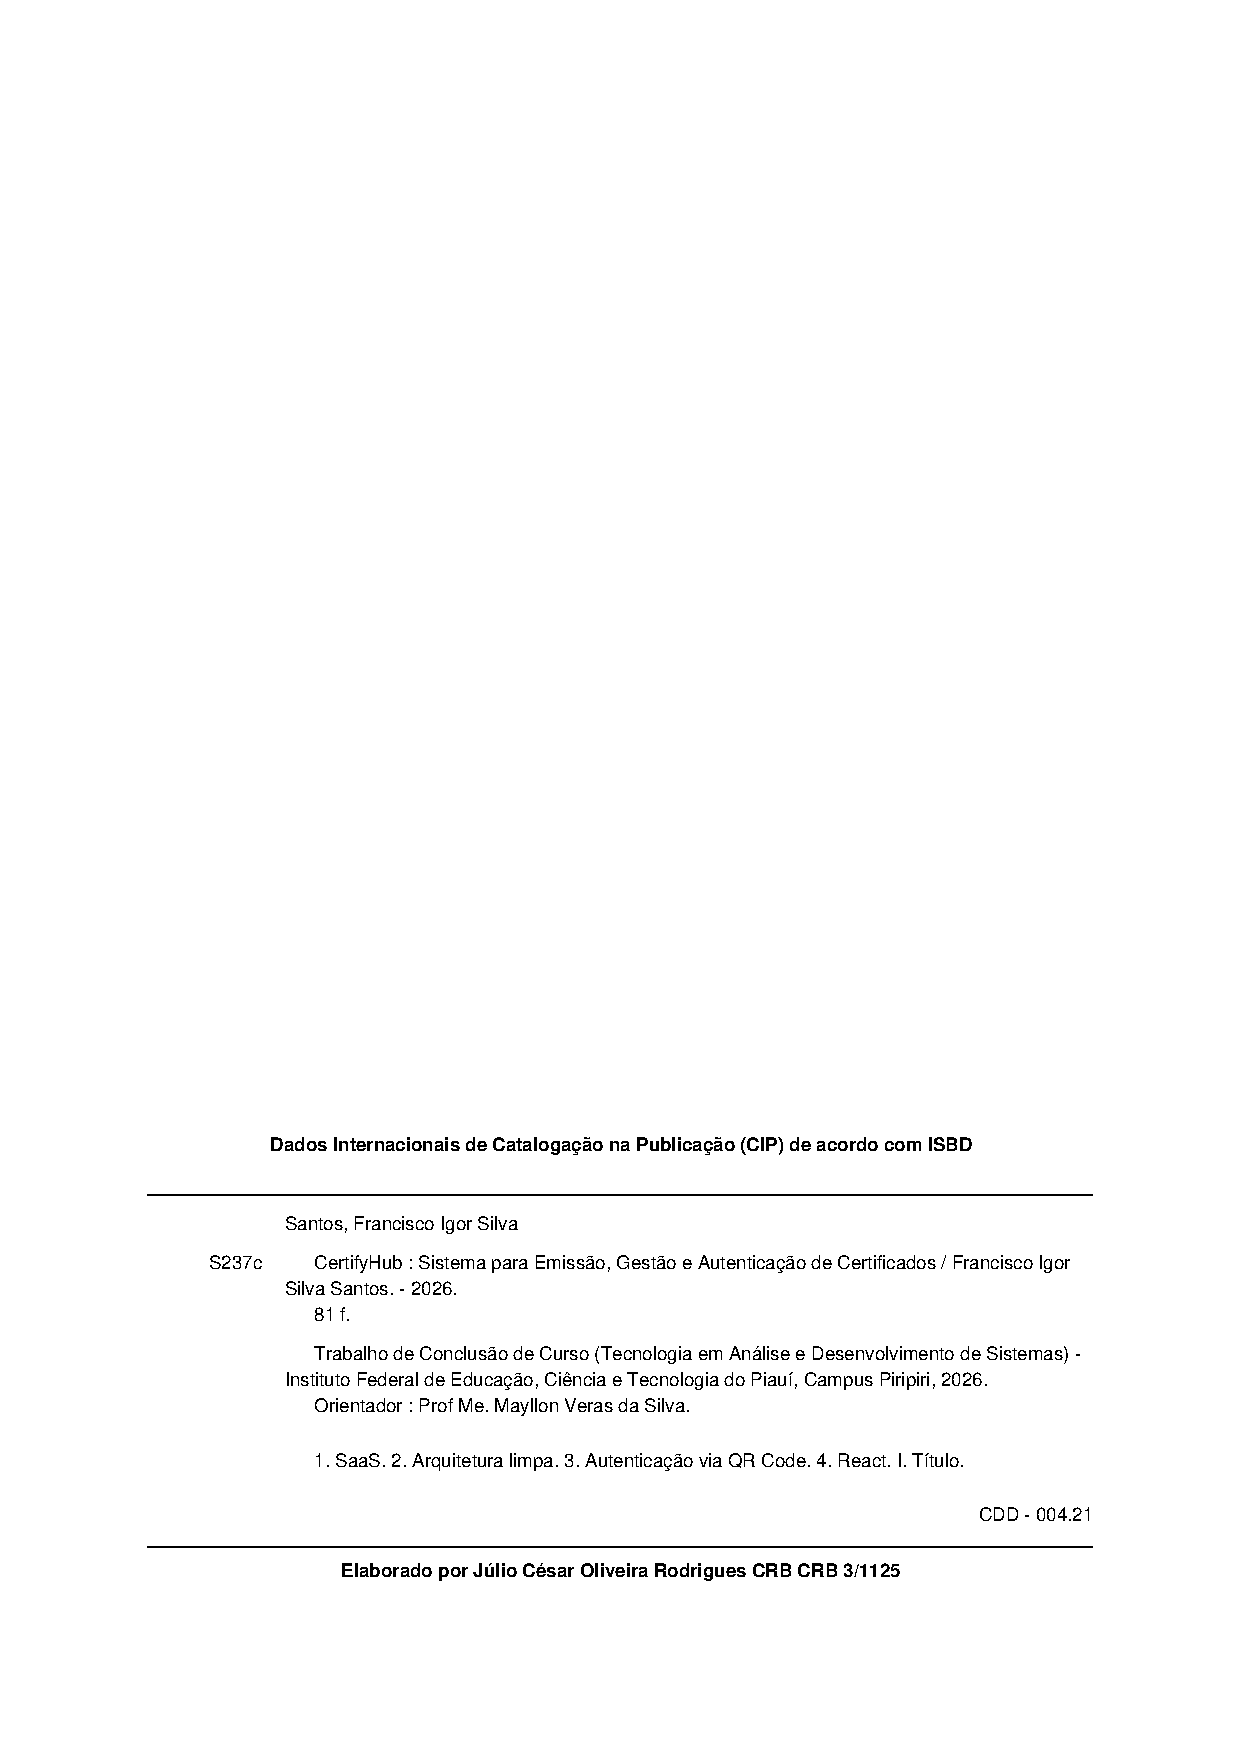
\includepdf[pages=-,pagecommand={\thispagestyle{pretextual}}]{anexos/ficha_catalografica.pdf}

% ================= CABEÇALHO PRÉ-RESUMO =================
\thispagestyle{pretextual}
\begin{center}
\textbf{\Titulo}
\end{center}

\vspace{1cm}

\begin{flushright}
\Autor \\
\Orientador
\end{flushright}

\vspace{1cm}

% ================= RESUMO E ABSTRACT =================
\thispagestyle{pretextual}
\begin{center}
\textbf{RESUMO}
\end{center}

Empresas de treinamento e instituições educacionais ainda dependem de processos manuais e soluções improvisadas para emissão de certificados, o que gera retrabalho, inconsistências e ausência de mecanismos confiáveis de validação. Este trabalho apresenta o desenvolvimento de um sistema web no modelo SaaS (\textit{Software as a Service}) para emissão, gestão e autenticação pública de certificados. A solução adota uma arquitetura desacoplada estruturada em duas aplicações independentes: um \textit{frontend} do tipo \textit{Single Page Application} (SPA) desenvolvido com React e TypeScript, e um \textit{backend} (Next.js) orientado aos princípios da Arquitetura Limpa, organizado nas camadas de apresentação, aplicação, domínio e infraestrutura. A persistência de dados ocorre em um banco relacional (PostgreSQL), enquanto a geração de PDFs é processada no servidor. As funcionalidades implementadas incluem \textit{templates} configuráveis com editor visual, emissão individual com código único e \textit{QR Code}, \textit{dashboard} gerencial e portal público de validação. O ciclo de vida da aplicação conta com \textit{pipeline} de CI/CD para integração e implantação contínuas em nuvem. A qualidade do software foi atestada por uma robusta suíte de testes automatizados (290 testes), alcançando cobertura de código de 82,6\% no \textit{frontend} e 96,53\% no \textit{backend} (medidos por \textit{Statements}). Conclui-se que o produto, na forma de um Produto Mínimo Viável (MVP) funcional e testado, atingiu os objetivos propostos, superando as restrições do fluxo manual por meio de uma plataforma escalável e segura.

\noindent\textbf{Palavras-chave:} emissão de certificados; SaaS; arquitetura limpa; React; autenticação via \textit{QR Code}.

\newpage
\begin{center}
\textbf{ABSTRACT}
\end{center}

Training companies and educational institutions still rely on manual processes and improvised solutions for certificate issuance, leading to rework, inconsistencies, and a lack of reliable validation mechanisms. This work presents the development of a SaaS (\textit{Software as a Service}) web system for issuing, managing, and publicly authenticating certificates. The solution adopts a decoupled architecture structured in two independent applications: a \textit{Single Page Application} (SPA) frontend developed with React and TypeScript, and a backend (Next.js) oriented towards Clean Architecture principles, organized into presentation, application, domain, and infrastructure layers. Data persistence is handled by a relational database (PostgreSQL), while PDF generation is processed on the server-side. Implemented features include configurable templates with a visual editor, individual issuance with unique codes and \textit{QR Codes}, a management dashboard, and a public validation portal. The application lifecycle is supported by a CI/CD pipeline for \textit{continuous integration} and cloud deployment. Software quality was ensured by a robust automated testing suite (290 tests), achieving 82.6\% code coverage on the frontend and 96.53\% on the backend (measured by \textit{Statements}). It is concluded that the product, as a functional and tested \textit{Minimum Viable Product} (MVP), achieved the proposed objectives, overcoming the constraints of the manual workflow through a scalable and secure platform.

\noindent\textbf{Keywords:} certificate issuance; SaaS; clean architecture; React; \textit{QR Code} authentication.

\vspace{1cm}

\noindent\textbf{Data de aprovação:} 15/07/2026

\vfill

\noindent\rule{5cm}{0.4pt}

{\small\noindent 1 Acadêmico do curso de Tecnólogo em Análise e Desenvolvimento de Sistemas pelo Instituto Federal do Piauí -- IFPI, Campus Piripiri.\\
\noindent 2 Mestre em Engenharia de Software pelo Centro de Estudos e Sistemas Avançados do Recife -- CESAR School. Professor de Ensino Superior e Professor do Ensino Básico, Técnico e Tecnológico do Instituto Federal do Piauí -- IFPI, Campus Piripiri.}

% ================= LISTA DE FIGURAS =================
\newpage
\thispagestyle{pretextual}
\listoffigures

% ================= LISTA DE QUADROS =================
\newpage
\thispagestyle{pretextual}
\listof{quadro}{LISTA DE QUADROS}

% ================= LISTA DE TABELAS =================
\newpage
\thispagestyle{pretextual}
\listoftables

% ================= LISTA DE ABREVIATURAS E SIGLAS =================
\newpage
\thispagestyle{pretextual}
\begin{center}
\textbf{LISTA DE ABREVIATURAS E SIGLAS}
\end{center}

\footnotesize
\renewcommand{\arraystretch}{0.85}
\begin{tabular}{@{}p{2.2cm}p{10.5cm}@{}}
API & \textit{Application Programming Interface} \\
BaaS & \textit{Backend as a Service} \\
CI/CD & \textit{Continuous Integration / Continuous Deployment} \\
CPF & Cadastro de Pessoa Física \\
CRUD & \textit{Create, Read, Update, Delete} \\
CORS & \textit{Cross-Origin Resource Sharing} \\
CSS & \textit{Cascading Style Sheets} \\
CT & Caso de Teste \\
CSV & \textit{Comma-Separated Values} \\
DDD & \textit{Domain-Driven Design} \\
DER & Diagrama Entidade-Relacionamento \\
DTO & \textit{Data Transfer Object} \\
E2E & \textit{End-to-End} \\
HMR & \textit{Hot Module Replacement} \\
HTML & \textit{HyperText Markup Language} \\
HTTP & \textit{Hypertext Transfer Protocol} \\
HTTPS & \textit{Hypertext Transfer Protocol Secure} \\
IFPI & Instituto Federal do Piauí \\
JSON & \textit{JavaScript Object Notation} \\
JWT & \textit{JSON Web Token} \\
LGPD & Lei Geral de Proteção de Dados \\
MFA & \textit{Multi-Factor Authentication} \\
MVP & \textit{Minimum Viable Product} \\
NIT & Núcleo de Inovação Tecnológica \\
ORM & \textit{Object-Relational Mapping} \\
OWASP & \textit{Open Web Application Security Project} \\
PDF & \textit{Portable Document Format} \\
PNG & \textit{Portable Network Graphics} \\
QR Code & \textit{Quick Response Code} \\
RBAC & \textit{Role-Based Access Control} \\
REST & \textit{Representational State Transfer} \\
RLS & \textit{Row Level Security} \\
SaaS & \textit{Software as a Service} \\
SDK & \textit{Software Development Kit} \\
SEO & \textit{Search Engine Optimization} \\
SMTP & \textit{Simple Mail Transfer Protocol} \\
SPA & \textit{Single Page Application} \\
SQL & \textit{Structured Query Language} \\
SSR & \textit{Server-Side Rendering} \\
SVG & \textit{Scalable Vector Graphics} \\
TLS & \textit{Transport Layer Security} \\
UC & Caso de Uso \\
URL & \textit{Uniform Resource Locator} \\
UUID & \textit{Universally Unique Identifier} \\
WCAG & \textit{Web Content Accessibility Guidelines} \\
\end{tabular}
\normalsize


% ================= SUMÁRIO =================
\newpage
\thispagestyle{pretextual}
\bgroup
\renewcommand{\contentsname}{}
\begin{center}
\textbf{SUMÁRIO}
\end{center}
\tableofcontents
\egroup
\newpage

% ================= CONTEÚDO =================
\renewcommand{\thepage}{\arabic{page}}
\pagestyle{fancy}
\fancyhf{}
\fancyhead[R]{\thepage}
\renewcommand{\headrulewidth}{0pt}
\thispagestyle{fancy}

% INTRODUÇÃO
\section{INTRODUÇÃO}

A emissão de certificados é uma atividade essencial para empresas de treinamentos, consultorias e instituições educacionais que promovem cursos, capacitações e eventos \cite{rahman2026,kulkarni2025}. Apesar da relevância desse processo, grande parte das organizações ainda depende de procedimentos manuais ou soluções improvisadas, utilizando ferramentas como Google Planilhas, Google Docs, PowerPoint e complementos externos.

Essas práticas resultam em retrabalho, inconsistências, falta de padronização e dificuldade de controle operacional. Além disso, ferramentas como AutoCrat \cite{autocrat2025} e documentos espalhados entre diferentes plataformas não foram projetados para uso profissional em escala, o que gera limitação, fragilidade e risco de inconsistências.

A ausência de um sistema integrado compromete a rastreabilidade e a credibilidade dos certificados, uma vez que não há mecanismos oficiais de validação pública, histórico centralizado, indicadores gerenciais ou emissão em lote eficiente. Estudos têm mostrado que sistemas baseados em \textit{QR Code} têm se destacado como alternativa eficaz para verificação de credenciais acadêmicas \cite{rahman2026}, combinando criptografia e códigos bidimensionais para garantir a autenticidade dos documentos \cite{wellem2021}. Esse cenário se agrava com o crescimento de cursos online e da necessidade de certificação confiável.

Diante disso, justifica-se o desenvolvimento de uma solução centralizada e automatizada, capaz de reduzir erros humanos, otimizar o tempo operacional e garantir segurança, conformidade e profissionalismo. Recursos como códigos únicos, validação via \textit{QR Code} e assinaturas digitais ampliam a confiabilidade dos certificados e fortalecem a imagem institucional das organizações emissoras \cite{kulkarni2025}.

Diante desse contexto, realizou-se uma análise de soluções existentes no mercado. No espectro open-source, o TrueCert \cite{truecert2025} oferece stack similar (React + Node.js), mas utiliza MongoDB e Express.js sem seguir Arquitetura Limpa, CI/CD ou testes automatizados. Já soluções brasileiras como AutoCert \cite{autocert2025} operam sobre Google Sheets, sem aplicação web própria. Nenhuma dessas alternativas combina simultaneamente código aberto, banco relacional, pipeline de CI/CD com cobertura superior a 82\% e arquitetura baseada nos princípios da Arquitetura Limpa, como proposto neste trabalho. Ressalta-se que uma ampla busca bibliográfica foi realizada em bases de dados nacionais (CAPES, SciELO, BDTD e Google Acadêmico com filtros para língua portuguesa) com o intuito de identificar trabalhos correlatos de cunho nacional abordando sistemas de emissão e validação de certificados com arquitetura web moderna; entretanto, não foram encontrados estudos que contemplassem simultaneamente os mesmos pilares técnicos propostos neste trabalho -- o que reforça a originalidade e a pertinência da presente contribuição.

O presente trabalho consiste no desenvolvimento de um Sistema Web -- produto do tipo SaaS (\textit{Software as a Service}) com arquitetura multi-tenant -- destinado à emissão, gestão e autenticação de certificados. O escopo do projeto foi definido a partir de um estudo de caso realizado em uma organização do ramo de treinamentos corporativos, por meio de entrevistas semiestruturadas e observação direta dos processos de emissão vigentes. As dificuldades identificadas -- como o tempo elevado para emissão manual, a dificuldade em gerenciar grandes volumes de certificados e a ausência de mecanismos de validação pública -- serviram como base para a definição dos requisitos funcionais e não funcionais do sistema. Dessa forma, o escopo abrange desde a automatização da criação e personalização de certificados até a disponibilização de um portal público de validação, visando substituir processos manuais por uma plataforma profissional, segura e escalável. Os direitos de propriedade intelectual do software desenvolvido são de propriedade do Instituto Federal do Piauí (IFPI).

O desenvolvimento seguiu a abordagem de Produto Mínimo Viável (MVP), priorizando as funcionalidades essenciais para a operação do sistema -- emissão de certificados, templates configuráveis, dashboard e validação pública -- enquanto funcionalidades complementares, como importação em lote e envio automático por e-mail, foram postergadas para versões futuras. O modelo SaaS adotado permite que o sistema seja oferecido como serviço centralizado, simplificando a manutenção, a escalabilidade e a atualização contínua da plataforma.

Este relatório técnico está organizado da seguinte forma: a Seção 2 apresenta as tecnologias utilizadas no desenvolvimento; a Seção 3 descreve a modelagem do sistema, incluindo levantamento de requisitos, diagramas de casos de uso, classes, arquitetura e entidade-relacionamento; a Seção 4 detalha a implementação do software; e a Seção 5 traz as considerações finais.

\subsection{OBJETIVOS}\label{sec:objetivos}

Os objetivos deste trabalho estão organizados em um objetivo geral e em objetivos específicos. O objetivo geral sintetiza a finalidade central do sistema proposto, enquanto os objetivos específicos detalham, de forma objetiva e mensurável, as metas técnicas e funcionais cuja realização é necessária para a concretização do projeto. Em conjunto, eles orientam a condução das etapas de levantamento de requisitos, modelagem, implementação e validação descritas ao longo deste relatório técnico.

\subsubsection{Geral}\label{sec:objetivo-geral}

Projetar e implementar um sistema web automatizado para emissão, gestão e validação de certificados, com base projetada para suporte a envio automático por e-mail em versões futuras, destinado a empresas de treinamento corporativo, instituições educacionais e demais organizações que necessitem certificar participantes em cursos, capacitações e eventos, a fim de eliminar a dependência de processos manuais e soluções improvisadas, garantindo padronização dos documentos, rastreabilidade do histórico de emissões, autenticação confiável via código único e \textit{QR Code}, centralização dos dados em uma única plataforma e estabelecendo as bases para emissão em lote eficiente em versões futuras.

\subsubsection{Específicos}\label{sec:objetivos-especificos}

\begin{itemize}
    \item implementar um módulo de templates configuráveis para a criação de certificados;
    \item desenvolver um mecanismo de autenticação pública via código único e \textit{QR Code} para garantir a integridade dos certificados e prevenir fraudes;
    \item desenvolver um módulo de dashboard com indicadores gerenciais para apoiar o controle operacional e a tomada de decisão das organizações sobre suas emissões, dispondo de filtros por período, curso e status;
    \item planejar e executar testes unitários e de integração para validação dos módulos implementados;
    \item configurar o ambiente de implantação do sistema em infraestrutura em nuvem com deploys automáticos a partir do repositório Git;
    \item projetar as bases conceituais e estruturais para conformidade com a LGPD, incluindo a modelagem do registro de consentimento, diretrizes para anonimização de dados pessoais, controle de acesso a logs sensíveis e trilha de auditoria para operações críticas, a serem refinadas em versões futuras;
    \item projetar a arquitetura multi-tenant do sistema, estabelecendo as bases conceituais para isolamento de dados entre organizações, segurança por tenant e escalabilidade horizontal em versões futuras.
\end{itemize}

% TECNOLOGIAS
\section{Tecnologias Envolvidas}
Descrição das linguagens, frameworks, banco de dados e ferramentas utilizadas no desenvolvimento e implantação do sistema.


\begin{table}[H]
\centering
\caption{Tecnologias utilizadas}
\begin{tabular}{@{}ll@{}}
\toprule
\textbf{Tecnologia} & \textbf{Descrição} \\
\midrule
React 19 & Desenvolvimento da interface do usuário (Frontend) \\
TypeScript & Linguagem de programação com tipagem estática \\
Tailwind CSS & Estilização da interface \\
TanStack React Router & Gerenciamento de rotas \\
TanStack React Query & Gerenciamento de estado assíncrono e cache \\
Node.js & Ambiente de execução do backend \\
Next.js & Framework para API e funcionalidades do servidor \\
Supabase & Plataforma de banco de dados e autenticação \\
PostgreSQL & Sistema de gerenciamento de banco de dados relacional \\
Zod & Validação de dados \\
PDFKit & Geração de certificados em PDF \\
Jest & Testes unitários e de integração \\
Docker & Conteinerização da aplicação \\
Render & Hospedagem e deploy do frontend e backend \\
Git & Controle de versão do código-fonte \\
GitHub & Repositório remoto e colaboração da equipe \\
Visual Studio Code & Ambiente de Desenvolvimento Integrado (IDE) \\
Vite & Ferramenta de build e desenvolvimento frontend \\
\bottomrule
\end{tabular}
\end{table}

% MODELAGEM
\section{Modelagem do Projeto}
\subsection{Levantamento de Requisitos}
\label{sec:requisitos}

O levantamento de requisitos foi realizado por meio de uma entrevista semiestruturada com o responsável pela emissão de certificados na instituição parceira, juntamente com a observação direta do processo manual executado por ele. Durante a entrevista, foram identificadas as principais dificuldades enfrentadas, como o tempo elevado para emissão manual, a dificuldade em gerenciar grandes volumes de certificados e a ausência de um mecanismo de validação pública. A análise do processo permitiu mapear o fluxo completo de emissão, desde o cadastro de participantes até a entrega do certificado, servindo como base para a definição dos requisitos funcionais e não funcionais apresentados a seguir.


\textbf{Requisitos Funcionais}:

\subsubsection{Módulo de Autenticação e Controle de Acesso}
\begin{itemize}
\item RF001 – Permitir login por e-mail e senha.
\item RF002 – Permitir redefinição de senha via e-mail.
\item RF003 – Validar credenciais antes de conceder acesso.
\item RF004 – Permitir cadastro de novos usuários (apenas administrador).
\item RF005 – Permitir gerenciamento de perfis e permissões.
\item RF006 – Controlar acesso a áreas restritas com base no status de autenticação do usuário.
\item RF007 – Controlar sessões ativas por conta, permitindo apenas uma sessão simultânea.
\end{itemize}

\subsubsection{Módulo de Templates de Certificados}
\begin{itemize}
\item RF008 – Permitir upload de templates (PPTX, DOCX, PDF).
\item RF009 – Permitir personalização de templates.
\item RF010 – Permitir selecionar template da galeria interna.
\item RF011 – Identificar campos dinâmicos automaticamente.
\item RF012 – Permitir criação/edição manual de campos dinâmicos (ex: \{\{nome\}\}).
\item RF013 – Salvar configurações de mapeamento de campos.
\item RF014 – Permitir duplicar templates existentes.
\end{itemize}

\subsubsection{Módulo de Entrada de Dados}
\begin{itemize}
\item RF015 – Permitir cadastro individual de participantes.
\item RF016 – Permitir emissão manual para participante único.
\item RF017 – Importar dados via CSV.
\item RF018 – Importar dados via Excel (.xlsx).
\item RF019 – Configurar gatilhos de emissão automática.
\item RF020 – Permitir upload de lista em lote.
\item RF021 – Processar múltiplos certificados em fila.
\item RF022 – Notificar ao término do processamento.
\end{itemize}

\subsubsection{Módulo de Geração de Certificados}
\begin{itemize}
\item RF023 – Gerar certificados em PDF.
\item RF024 – Preencher automaticamente campos dinâmicos.
\item RF025 – Gerar código único por certificado.
\item RF026 – Registrar data, hora e localidade da emissão.
\item RF027 – Permitir reemissão mantendo histórico.
\item RF028 – Permitir download individual.
\item RF029 – Permitir download em lote.
\end{itemize}

\subsubsection{Módulo de Envio e Comunicação}
\begin{itemize}
\item RF030 – Permitir personalização do corpo do e-mail com variáveis.
\item RF031 – Registrar status de envio (pendente, enviado, falha).
\item RF032 – Reenviar automaticamente em caso de falha (até 3 tentativas a cada 10 min).
\end{itemize}

\subsubsection{Módulo de Validação Pública e Antifraude}
\begin{itemize}
\item RF033 – Disponibilizar portal público de validação.
\item RF034 – Validar certificado via código único.
\item RF035 – Gerar QR Code no certificado.
\item RF036 – Permitir personalização de cores do QR Code.
\item RF037 – Exibir informações básicas ao validar (nome, curso, data, validade, autenticidade).
\end{itemize}

\subsubsection{Módulo de Assinaturas Digitais}
\begin{itemize}
\item RF038 – Permitir adicionar assinatura digitalizada ao template.
\item RF039 – Registrar hash de verificação da assinatura.
\end{itemize}

\subsubsection{Módulo de Dashboard e Gestão}
\begin{itemize}
\item RF040 – Exibir lista completa de certificados emitidos.
\item RF041 – Permitir filtros por curso, período, status e instrutor.
\item RF042 – Exibir estatísticas mensais de emissão.
\item RF043 – Exibir logs de ações realizadas.
\end{itemize}

\subsubsection{Módulo de Auditoria e Segurança Operacional}
\begin{itemize}
\item RF044 – Registrar responsável por cada certificado gerado.
\item RF045 – Registrar data, hora e local de ações relevantes.
\item RF046 – Permitir arquivamento de certificados como alternativa à exclusão definitiva.
\end{itemize}

\subsubsection{Módulo de Gestão de Cursos/Eventos}
\begin{itemize}
\item RF047 – Permitir cadastro de cursos/eventos.
\item RF048 – Associar participantes ao curso.
\item RF049 – Definir carga horária.
\item RF050 – Registrar instrutor responsável.
\item RF051 – Configurar datas de início e término.
\item RF052 – Listar certificados vinculados ao curso.
\item RF053 – Validar vínculo do participante ao curso antes de permitir a emissão.
\item RF054 – Registrar local do curso.
\end{itemize}

\subsubsection{Módulo de Participantes}
\begin{itemize}
\item RF055 – Cadastro completo de participantes (nome, e-mail, CPF opcional).
\item RF056 – Permitir edição de dados.
\item RF057 – Importar participantes sem duplicidade.
\item RF058 – Exibir histórico de certificados por participante.
\item RF059 – Permitir busca por nome, e-mail e CPF.
\end{itemize}

\subsubsection{Módulo Multiempresa / Multi-tenant}
\begin{itemize}
\item RF060 – Permitir cadastro de múltiplas organizações.
\item RF061 – Isolar dados entre organizações.
\item RF062 – Permitir que cada empresa tenha seus próprios templates.
\item RF063 – Permitir que administradores gerenciem usuários internos.
\end{itemize}

\subsubsection{Módulo de Configurações do Sistema}
\begin{itemize}
\item RF064 – Personalizar mensagens padrão.
\item RF065 – Ativar/desativar envio automático.
\item RF066 – Configurar regras de reemissão.
\end{itemize}

\subsubsection{Módulo de Armazenamento e Arquivos}
\begin{itemize}
\item RF067 – Permitir exclusão lógica (soft-delete) de arquivos.
\item RF068 – Armazenar templates no sistema.
\end{itemize}

\subsubsection{Módulo de Notificações e Alertas}
\begin{itemize}
\item RF069 – Notificar falhas de emissão.
\item RF070 – Notificar sucesso no processamento de planilhas.
\item RF071 – Alertar quando template estiver incompleto ou inválido.
\end{itemize}

\subsubsection{Módulo de Monitoramento e Logs}
\begin{itemize}
\item RF072 – Registrar logs de autenticação e tentativas de acesso.
\item RF073 – Registrar eventos críticos (falha geração PDF etc.).
\item RF074 – Permitir exportação de logs.
\end{itemize}

\subsubsection{Módulo de Suporte, Operação e Manutenção}
\begin{itemize}
\item RF075 – Permitir abertura de chamados de suporte.
\item RF076 – Exibir status do sistema (online/manutenção).
\item RF077 – Permitir atualização de termos de uso e políticas.
\end{itemize}
\vspace{1em}
\textbf{Requisitos Não Funcionais}:

Os requisitos não funcionais foram priorizados segundo o método MoSCoW, alinhado à abordagem MVP (Produto Mínimo Viável) adotada no projeto: \textbf{[M]} \textit{Must have} — requisitos essenciais implementados no MVP; \textbf{[S]} \textit{Should have} — importantes, mas não críticos para a primeira versão; \textbf{[C]} \textit{Could have} — desejáveis para versões futuras; \textbf{[W]} \textit{Won't have} — fora do escopo do MVP.

\subsubsection{Segurança}
\begin{itemize}
\rnfitem{rnf:supabase-auth}{[S] O sistema deve utilizar o Supabase Auth para gerenciamento seguro de autenticação e armazenamento de senhas com hash criptográfico seguro (bcrypt).}
\rnfitem{rnf:https}{[M] O sistema deve utilizar conexão segura HTTPS (TLS 1.2 ou superior) em todas as comunicações entre o cliente e o servidor, garantindo confidencialidade e integridade dos dados em trânsito.}
\rnfitem{rnf:encryption-at-rest}{[S] O sistema deve proteger dados sensíveis em repouso utilizando criptografia fornecida pela infraestrutura em nuvem.}
\rnfitem{rnf:login-attempt-limit}{[S] O sistema deve bloquear autenticação após 5 tentativas consecutivas inválidas (conforme política do provedor de autenticação).}
\rnfitem{rnf:session-timeout}{[C] Sessões inativas devem expirar automaticamente após tempo configurável (ex.: 30 minutos).}
\rnfitem{rnf:rbac}{[M] O sistema deve implementar controle de acesso baseado em papéis (RBAC).}
\rnfitem{rnf:owasp}{[S] O sistema deve seguir boas práticas de segurança conforme OWASP Top 10.}
\rnfitem{rnf:auth-logs}{[S] O sistema deve registrar logs de autenticação e eventos de segurança, incluindo tentativas de login, falhas, acessos negados e alterações de configuração, com data, hora e identificação do usuário.}
\rnfitem{rnf:tenant-isolation}{[C] O sistema deve garantir isolamento de dados entre empresas (multi-tenant).}
\rnfitem{rnf:mfa}{[W] O sistema deve permitir futura implementação de autenticação multifator (MFA).}
\rnfitem{rnf:emission-schedules}{[C] O sistema deve permitir configurar horários de emissão por perfil de colaborador como política de segurança.}
\end{itemize}

\subsubsection{Desempenho e Escalabilidade}

Os valores numéricos apresentados a seguir são estimativas definidas pelo desenvolvedor com base no porte esperado da operação, considerando turmas típicas de 20 a 50 participantes, palestras com até 200 participantes e emissões recorrentes ao longo do ano. Os limites estabelecidos consideram uma margem de segurança para absorver picos sazonais sem degradação da experiência do usuário.

\vspace{0.5em}
\begin{itemize}
\rnfitem{rnf:batch-capacity}{[M] O sistema deve suportar geração simultânea de, estimados, 500 certificados por lote, volume equivalente a duas turmas grandes ou dez turmas médias processadas em única operação.}
\rnfitem{rnf:generation-time}{[M] O tempo médio de geração individual não deve exceder 5 segundos por certificado, garantindo que um lote de 500 certificados seja concluído em aproximadamente 42 minutos.}
\rnfitem{rnf:validation-response-time}{[M] O portal público de validação deve responder em até 2 segundos.}
\rnfitem{rnf:horizontal-scaling}{[S] O sistema deve permitir escalabilidade horizontal do serviço de geração.}
\rnfitem{rnf:monthly-volume}{[S] O sistema deve suportar volume estimado de 10.000 certificados/mês, compatível com a projeção de emissões recorrentes acrescida de margem de segurança.}
\rnfitem{rnf:async-batch-processing}{[M] A geração em lote deve ser processada de forma assíncrona por meio de fila de processamento, sem bloquear a aplicação principal.}
\rnfitem{rnf:queue-ordering}{[S] A fila de certificados deve garantir processamento ordenado e controle de concorrência.}
\end{itemize}

\subsubsection{Disponibilidade e Confiabilidade}
\begin{itemize}
\rnfitem{rnf:uptime}{[S] O sistema deve garantir disponibilidade mínima de 99,5\% mensal.}
\rnfitem{rnf:daily-backup}{[S] O sistema deve realizar backup automático diário do banco de dados, com retenção mínima de 30 dias, garantindo recuperação de dados em caso de falha ou corrupção.}
\rnfitem{rnf:restore-time}{[C] O sistema deve permitir restauração de dados em até 24 horas.}
\rnfitem{rnf:retry-mechanism}{[S] O sistema deve implementar mecanismo de retentativa automática para tarefas falhas na fila de certificados.}
\rnfitem{rnf:failure-logging}{[M] O sistema deve registrar falhas de processamento para auditoria posterior.}
\end{itemize}

\subsubsection{Usabilidade e Acessibilidade}
\begin{itemize}
\rnfitem{rnf:responsive}{[M] O sistema deve ser responsivo (desktop, tablet e mobile).}
\rnfitem{rnf:visual-consistency}{[M] O sistema deve manter padrão visual consistente.}
\rnfitem{rnf:error-messages}{[M] O sistema deve fornecer mensagens de erro claras.}
\rnfitem{rnf:keyboard-nav}{[S] O sistema deve permitir navegação por teclado.}
\rnfitem{rnf:wcag}{[C] O sistema deve seguir recomendações WCAG 2.1 nível AA (quando aplicável).}
\end{itemize}

\subsubsection{Compatibilidade e Integração}
\begin{itemize}
\rnfitem{rnf:browser-compat}{[M] O sistema deve ser compatível com navegadores modernos (Chrome, Firefox, Edge, Safari).}
\rnfitem{rnf:pdf-fidelity}{[M] A geração de PDF deve preservar fidelidade visual do template original.}
\rnfitem{rnf:rest-api}{[M] O sistema deve disponibilizar API REST autenticada via token JWT do Supabase.}
\rnfitem{rnf:csv-utf8}{[S] O sistema deve aceitar arquivos CSV codificados em UTF-8.}
\rnfitem{rnf:webhooks}{[C] O sistema deve permitir integração via Webhooks em formato JSON.}
\end{itemize}

\subsubsection{Armazenamento e Retenção}
\begin{itemize}
\rnfitem{rnf:storage-retention}{[S] O sistema deve armazenar certificados de forma permanente, garantindo validação indefinida pelo portal público.}
\rnfitem{rnf:soft-delete}{[S] O sistema deve aplicar exclusão lógica (soft delete) quando aplicável.}
\end{itemize}

\subsubsection{Conformidade Legal e LGPD}
\begin{itemize}
\rnfitem{rnf:lgpd}{[C] O sistema deve estar em conformidade com a LGPD (Lei nº 13.709/2018), garantindo tratamento adequado dos dados pessoais coletados, incluindo consentimento, finalidade específica, minimização de dados e direitos do titular.}
\rnfitem{rnf:data-deletion}{[C] O sistema deve permitir exclusão ou anonimização de dados pessoais mediante solicitação.}
\rnfitem{rnf:consent-logging}{[C] O sistema deve registrar consentimento do usuário para o tratamento de dados pessoais, incluindo finalidade, base legal e data da coleta.}
\rnfitem{rnf:sensitive-logs}{[S] Logs sensíveis devem ser acessíveis apenas por administradores autorizados.}
\rnfitem{rnf:audit-trail}{[S] O sistema deve manter trilha de auditoria inviolável para operações críticas.}
\end{itemize}

\subsubsection{Arquitetura e Tecnologia}
\begin{itemize}
\rnfitem{rnf:independent-apps}{[M] O sistema deve ser composto por duas aplicações independentes: uma \textit{Single Page Application} (SPA) para o frontend e uma API REST para o backend, cada uma com seu próprio ciclo de vida de desenvolvimento e deploy.}
\rnfitem{rnf:frontend-layers}{[M] O frontend deve adotar arquitetura em camadas com React, com quatro camadas: (i) \textit{View} --- componentes de interface; (ii) \textit{ViewModel} --- custom hooks que encapsulam estado e ações; (iii) \textit{Service} --- cliente de comunicação com a API; (iv) \textit{Model} --- interfaces TypeScript que definem as entidades de domínio.}
\rnfitem{rnf:backend-layers}{[M] O backend deve adotar arquitetura em camadas (domínio, aplicação e infraestrutura), com as dependências apontando para a camada de domínio (princípio de inversão de dependências).}
\rnfitem{rnf:api-communication}{[M] A comunicação entre frontend e backend deve ocorrer exclusivamente via API REST sobre HTTPS, com autenticação baseada em token JWT.}
\rnfitem{rnf:async-cert-generation}{[S] A geração de certificados em lote deve ser processada de forma assíncrona por meio de fila de processamento, sem bloquear a aplicação principal.}
\rnfitem{rnf:postgresql}{[M] O sistema deve utilizar banco de dados relacional com integridade referencial (PostgreSQL), gerenciado pelo Supabase.}
\rnfitem{rnf:multi-tenant-strategy}{[C] O sistema deve implementar estratégia de isolamento multi-tenant (por schema ou coluna organizacional).}
\rnfitem{rnf:monitoring}{[S] O sistema deve implementar monitoramento e observabilidade centralizada (logs, métricas e rastreamento).}
\rnfitem{rnf:static-deploy}{[M] O frontend deve ser compilado como site estático e implantado em plataforma de hospedagem com deploy contínuo a partir do repositório Git.}
\rnfitem{rnf:backend-deploy}{[M] O backend deve ser implantado como serviço web independente em plataforma em nuvem compatível com Node.js.}
\rnfitem{rnf:extensibility}{[S] O sistema deve permitir extensibilidade, garantindo que novos módulos possam ser adicionados seguindo os mesmos padrões arquiteturais já estabelecidos.}
\end{itemize}

\subsubsection{Manutenção e Monitoramento}
\begin{itemize}
\rnfitem{rnf:zero-downtime-deploy}{[S] O sistema deve permitir atualização com mínima indisponibilidade (deploy contínuo).}
\rnfitem{rnf:documentation}{[M] O sistema deve possuir documentação técnica e manual do usuário.}
\rnfitem{rnf:error-monitoring}{[S] O sistema deve registrar erros em sistema centralizado de monitoramento.}
\rnfitem{rnf:backward-compatibility}{[S] O sistema deve permitir extensibilidade sem impacto nas funcionalidades existentes.}
\rnfitem{rnf:template-history}{[C] O sistema deve manter histórico de versões de templates, configurações e endpoints da API para fins de auditoria, rastreabilidade e versionamento.}
\end{itemize}

\subsubsection{Internacionalização}
\begin{itemize}
\rnfitem{rnf:timezone}{[S] O sistema deve permitir configuração de timezone por organização.}
\rnfitem{rnf:i18n}{[W] O sistema deve permitir tradução futura da interface.}
\rnfitem{rnf:date-format}{[C] O sistema deve suportar diferentes formatos de data e hora.}
\end{itemize}

\subsection{Regras de Negócio}

Além dos requisitos funcionais, foram identificadas regras de negócio que impõem restrições ou condições sobre as funcionalidades do sistema:

\begin{itemize}
\rnitem{rn:acesso-restrito}{Não deve ser permitido acesso a áreas restritas sem autenticação prévia.}
\rnitem{rn:certificado-arquivado}{Certificados não podem ser excluídos definitivamente, devendo ser arquivados.}
\rnitem{rn:vinculo-participante}{Certificados só podem ser emitidos para participantes previamente vinculados ao curso ou evento.}
\rnitem{rn:reenvio-limite}{O reenvio automático de certificados com falha deve respeitar o limite máximo de 3 tentativas com intervalo mínimo de 10 minutos entre cada uma.}
\end{itemize}

\subsubsection{Status de Implementação das Regras de Negócio}

As regras de negócio acima representam o modelo completo desejado para o sistema. No entanto, considerando o escopo do MVP (v1.0), algumas regras ainda não foram implementadas:

\begin{itemize}
\item \textbf{rn:certificado-arquivado} --- No MVP atual, a exclusão de templates e certificados é realizada por exclusão definitiva (\textit{hard delete}), conforme testado nos casos CT005 e CT056 do plano de testes. A regra de arquivamento (\textit{soft delete}) está prevista para a versão 2.0, conforme o requisito \ref{rf:arquivamento-certificados} [S].
\item \textbf{rn:vinculo-participante} --- A validação de vínculo entre participante e curso não é verificada no MVP, pois as entidades Participantes e Cursos ainda não foram materializadas no banco de dados.
\item \textbf{rn:reenvio-limite} --- O reenvio automático com limite de tentativas não foi implementado no MVP; o envio de e-mails é simulado sem controle de retentativas.
\end{itemize}

A implementação completa dessas regras está vinculada aos requisitos classificados como [S] ou [C], que serão tratados em versões futuras do sistema.


\subsection{Critérios de Aceitação}

Cada requisito funcional possui critérios de aceitação que definem as condições necessárias para considerá-lo atendido. A Tabela~\ref{tab:criterios} apresenta os critérios para todos os RFs.

\renewcommand{\arraystretch}{0.9}
\small
\begin{longtable}{p{1cm} p{3.2cm} p{10.8cm}}
\caption{Critérios de aceitação dos requisitos funcionais}
\label{tab:criterios}\\
\toprule
\textbf{RF} & \textbf{Descrição} & \textbf{Critério de Aceitação} \\
\midrule
\endfirsthead
\toprule
\textbf{RF} & \textbf{Descrição} & \textbf{Critério de Aceitação} \\
\midrule
\endhead
\bottomrule
\endfoot
\bottomrule
\endlastfoot
RF001 & Login por e-mail e senha & Usuário com credenciais válidas acessa o sistema; credenciais inválidas exibem mensagem de erro sem redirecionar. \\
RF002 & Redefinição de senha & Usuário clica em "Esqueci senha", insere e-mail e recebe link de redefinição válido por 1 hora. \\
RF003 & Validar credenciais & Rotas protegidas redirecionam para login quando o usuário não está autenticado; API retorna 401 para requisições sem token. \\
RF004 & Cadastro de usuários & Apenas administrador pode acessar tela de cadastro; formulário exige nome, e-mail e senha; usuário criado aparece na lista. \\
RF005 & Gerenciar perfis & Administrador pode listar, criar, editar e desativar usuários; alterações persistem após recarregar. \\
RF006 & Controle de acesso & Usuário não autenticado é redirecionado para login ao acessar qualquer rota administrativa. \\
RF007 & Sessão única & Login em novo dispositivo invalida sessão anterior; sessão expira após 30 min de inatividade. \\
\midrule
RF008 & Upload de templates & Arquivos .pptx e .pdf são aceitos; formatos .exe, .zip são rejeitados com mensagem clara; template aparece na galeria após upload. \\
RF009 & Personalização & Cores, fontes e bordas configuradas são refletidas no preview visual. \\
RF010 & Selecionar template & Galeria exibe templates salvos com nome e preview; seleção carrega o template para edição. \\
RF011 & Identificar campos automáticos & Sistema sugere campos \{\{nome\}\}, \{\{curso\}\} ao fazer upload; sugestões são editáveis. \\
RF012 & Criar/editar campos & Usuário adiciona campo \{\{cpf\}\}, salva, e o campo aparece na tela de emissão. \\
RF013 & Salvar configurações & Mapeamento de campos persiste após recarregar a página. \\
RF014 & Duplicar templates & Duplicata cria cópia idêntica com nome "(cópia)"; original não é alterado. \\
\midrule
RF015 & Cadastro individual & Formulário válido salva participante; e-mail duplicado exibe alerta; participante aparece na lista. \\
RF016 & Emissão manual & Selecionar template, preencher dados e confirmar gera certificado listado no dashboard. \\
RF017 & Importar CSV & Arquivo CSV com cabeçalho correto importa participantes; linhas com erro são ignoradas e reportadas. \\
RF018 & Importar Excel & Arquivo .xlsx com abas é processado; primeira aba é usada como padrão. \\
RF019 & Gatilhos automáticos & Ao cadastrar participante em curso com gatilho ativo, certificado é emitido automaticamente em até 30s. \\
RF020 & Upload em lote & Arquivo com 100 participantes é processado; certificados são gerados para todos. \\
RF021 & Fila de processamento & Lote de 500 participantes é enfileirado; barra de progresso mostra andamento. \\
RF022 & Notificar término & Processamento concluído envia notificação na tela (toast) com resumo. \\
\midrule
RF023 & Gerar PDF & PDF gerado preserva layout, cores e fontes do template; campos preenchidos aparecem nas posições corretas; geração leva menos de 5 segundos. \\
RF024 & Preencher campos & Dados do participante substituem corretamente os \{\{placeholders\}\} no PDF. \\
RF025 & Código único & Cada certificado possui código único (UUID v4); consulta no banco retorna apenas um registro. \\
RF026 & Data/hora/local & Certificado exibe data e hora da emissão; localização é definida pelo curso ou configuração. \\
RF027 & Reemissão & Reemissão gera novo PDF com novo código; histórico lista versão anterior com data. \\
RF028 & Download individual & PDF é baixado com nome no formato \texttt{Nome\_Curso\_Data.pdf}. \\
RF029 & Download em lote & Selecionar múltiplos certificados e baixar gera arquivo .zip com todos os PDFs. \\
\midrule
RF030 & Personalizar e-mail & Variáveis \{\{nome\}\}, \{\{link\}\} são substituídas no corpo do e-mail enviado. \\
RF031 & Status de envio & Certificado exibe status "Pendente", "Enviado" ou "Falha"; status é atualizado em tempo real. \\
RF032 & Reenvio automático & Falha de envio dispara nova tentativa após 10 min, até 3 tentativas. \\
\midrule
RF033 & Portal de validação & URL pública \texttt{/validar} exibe campo para inserir código; página é responsiva. \\
RF034 & Validar via código & Código válido exibe dados do certificado; inválido mostra "Certificado não encontrado". \\
RF035 & QR Code & QR Code no PDF redireciona para URL de validação com código como parâmetro. \\
RF036 & Exibir informações & Tela de validação mostra nome, curso, data, carga horária e status "Autêntico". \\
\midrule
RF037 & Assinatura digitalizada & Imagem de assinatura aparece na posição configurada no template. \\
RF038 & Hash da assinatura & Hash SHA-256 da assinatura é armazenado e verificável. \\
\midrule
RF039 & Lista de certificados & Tabela exibe certificados com colunas: nome, curso, data, status; paginação de 20 itens. \\
RF040 & Filtros & Filtrar por curso, período, status e instrutor atualiza a tabela sem recarregar a página. \\
RF041 & Estatísticas mensais & Dashboard exibe total de emissões por mês em gráfico de barras; dados são atualizados automaticamente. \\
RF042 & Logs de ações & Tabela de logs exibe ação, usuário, data e detalhes; ordenada por data decrescente. \\
\midrule
RF043 & Responsável & Certificado gerado registra ID do usuário que emitiu; exibido no histórico. \\
RF044 & Data/hora ações & Toda ação de emissão, edição e exclusão registra timestamp. \\
RF045 & Arquivamento & Certificado arquivado não aparece na lista padrão, mas é recuperável via filtro "Arquivados". \\
\midrule
RF046 & Cadastro cursos & Formulário salva nome, tipo, carga horária, datas e instrutor; curso aparece na lista. \\
RF047 & Associar participantes & Participante é vinculado ao curso no momento da emissão. \\
RF048 & Carga horária & Carga horária definida no curso aparece no campo correspondente do certificado. \\
RF049 & Instrutor & Nome do instrutor é salvo e exibido no certificado. \\
RF050 & Configurar datas & Datas configuradas são preenchidas automaticamente no certificado. \\
RF051 & Listar por curso & Filtro "Curso" exibe apenas certificados daquele curso. \\
RF052 & Validar vínculo & Emissão é bloqueada se participante não pertence ao curso selecionado; mensagem exibe motivo. \\
RF053 & Registrar local & Local do curso é salvo e exibido no certificado. \\
\midrule
RF054 & Cadastro completo & Nome e e-mail são obrigatórios; CPF é opcional; e-mail inválido é rejeitado. \\
RF055 & Edição & Dados editados são salvos e refletidos na tela de emissão. \\
RF056 & Importar sem duplicidade & Mesmo CPF/e-mail não cria registro duplicado; dados existentes são atualizados. \\
RF057 & Histórico & Página do participante exibe todos os certificados emitidos para ele. \\
RF058 & Busca & Busca por nome retorna resultados em menos de 2s; busca vazia retorna lista completa. \\
\midrule
RF059 & Cadastro organizações & Formulário salva CNPJ, razão social e contato; organização aparece na lista. \\
RF060 & Associar user/org & Usuário é vinculado a uma organização no cadastro; vínculo é editável. \\
RF061 & Templates por org & Organização A não vê templates da organização B. \\
RF062 & Usuários por org & Organização A não vê usuários da organização B. \\
\midrule
RF063 & Mensagens padrão & Texto padrão de e-mail é configurável por organização. \\
RF064 & Envio automático & Opção "Enviar automaticamente" é ativável/desativável por organização. \\
RF065 & Regras de reemissão & Reemissão é permitida apenas se configurada; limite de reemissões é respeitado. \\
\midrule
RF066 & Armazenar templates & Template enviado fica imediatamente disponível para uso; download do template original é possível. \\
\midrule
RF067 & Notificar falhas & Falha de emissão dispara notificação ao administrador com detalhes do erro. \\
RF068 & Notificar sucesso & Processamento concluído com sucesso exibe toast com total de certificados. \\
RF069 & Alertar template inválido & Template sem campos \{\{nome\}\} exibe alerta antes da emissão. \\
\midrule
RF070 & Logs de autenticação & Tentativa de login com senha incorreta é registrada com timestamp e IP. \\
RF071 & Eventos críticos & Falha de geração de PDF é registrada com stack trace e ID do certificado. \\
RF072 & Exportar logs & Logs são exportáveis em CSV com filtro por período. \\
\midrule
RF073 & Chamados de suporte & Formulário de chamado salva descrição, prioridade e contato; chamado é listado. \\
RF074 & Status do sistema & Página de status exibe "Online", "Em manutenção" ou "Indisponível". \\
RF075 & Termos de uso & Atualização de termos exibe aviso para aceite na próxima autenticação. \\
\bottomrule
\end{longtable}
\normalsize
\renewcommand{\arraystretch}{1.0}


\subsection{Matriz de Rastreabilidade}

O Quadro~\ref{qua:rastreabilidade} apresenta a matriz de rastreabilidade que relaciona os requisitos funcionais implementados no MVP aos casos de uso, às principais classes do diagrama de classes e às tabelas do banco de dados, garantindo a rastreabilidade entre os artefatos do projeto. A tabela foi disposta em orientação vertical (rotacionada 90\textdegree) para preservar a legibilidade de seu conteúdo, uma vez que possui quatro colunas com textos extensos.

\clearpage
\begingroup
\renewcommand{\tablename}{Quadro}
\begin{sidewaystable}[p!]
\centering
\footnotesize
\captionsetup{type=quadro}
\caption{Matriz de rastreabilidade entre requisitos funcionais, casos de uso, classes e tabelas implementados no MVP}
\label{qua:rastreabilidade}
\setlength{\tabcolsep}{3pt}
\renewcommand{\arraystretch}{0.9}
\begin{tabularx}{\textwidth}{|>{\raggedright\arraybackslash}X|>{\raggedright\arraybackslash}X|>{\raggedright\arraybackslash}X|>{\raggedright\arraybackslash}X|}
\hline
\textbf{Módulo / RFs} & \textbf{Casos de Uso} & \textbf{Classes} & \textbf{Tabelas} \\
\hline
Templates de Certificados (\ref{rf:upload-templates}–\ref{rf:mapeamento-campos}) & Gerenciar Templates (UC002), Criar Template, Editar Template, Salvar Template & Template, TemplateLayout & TEMPLATES \\
\hline
Entrada de Dados e Emissão (\ref{rf:cadastro-participante}, \ref{rf:emissao-manual}) & Emitir Certificado Individual (UC004) & Certificate, EmitCertificateUseCase, ICertificateRepository & CERTIFICADOS \\
\hline
Geração de Certificados (\ref{rf:gerar-pdf}–\ref{rf:download-individual}) & Emitir Certificado (UC004), Gerar PDF, Obter Certificado & Certificate, VerificationCode, EmitCertificateUseCase, GeneratePDFUseCase, GetCertificateUseCase, ICertificateRepository, ITemplateRepository, IPDFService, SupabaseCertificateRepository, SupabaseTemplateRepository, PDFKitService & CERTIFICADOS \\
\hline
Validação Pública (\ref{rf:portal-validacao}–\ref{rf:exibir-validacao}) & Validar Certificado (UC008) & VerifyCertificateUseCase, VerifyResult, Certificate (Frontend) & CERTIFICADOS \\
\hline
Dashboard e Gestão (\ref{rf:lista-certificados}–\ref{rf:estatisticas-emissao}) & Visualizar Dashboard (UC014) & Certificate (Frontend), Template (Frontend) & CERTIFICADOS, TEMPLATES \\
\hline
Armazenamento de Templates (\ref{rf:armazenar-templates}) & Gerenciar Templates (UC002) & Template, SupabaseTemplateRepository & TEMPLATES \\
\hline
\end{tabularx}
\end{sidewaystable}
\par\vspace{4pt}
\begin{center}\small\textit{Fonte: Elaborado pelo Autor (2026).}\end{center}
\endgroup
\clearpage


\subsection{Diagramas de casos de uso}
\begin{figure}[H]
\centering
\resizebox{\textwidth}{!}{
\begin{tikzpicture}[
    scale=0.7,
    transform shape,
    actor/.style={rectangle, draw=black, fill=blue!20, rounded corners, minimum width=1.8cm, minimum height=0.7cm},
    usecase/.style={ellipse, draw=black, minimum width=2.5cm, minimum height=0.8cm, font=\small},
    include/.style={->, dashed, font=\tiny},
    assoc/.style={-},
    every node/.style={font=\small}
]

% Fronteira do sistema
\draw (-0.5,-8.5) rectangle (18,5) node[above left, font=\small\bfseries, inner sep=3pt] at (18,5) {Sistema de Certificados};

% Atores
\node[actor] (admin) at (-3,1.5) {Administrador};
\node[actor] (colab) at (-3,-1.5) {Colaborador};
\node[actor] (visit) at (-3,-5) {Visitante};

% Generalização: Administrador herda casos de uso do Colaborador
\draw[-{Triangle[open]}] (admin) -- (colab);

% Casos Admin
\node[usecase, fill=red!20] (usuarios) at (2.5,3.5) {Gerenciar Usuários};
\node[usecase, fill=red!20] (template) at (2.5,1.8) {Criar Template};
\node[usecase, fill=red!20] (cursos) at (2.5,0) {Gerenciar Cursos};

\node[usecase, fill=yellow!30] (permissoes) at (7.5,3.5) {Definir Permissões};
\node[usecase, fill=red!20] (campos) at (7.5,1.8) {Configurar Campos};
\node[usecase, fill=red!20] (editar) at (7.5,0) {Editar Template};

\node[usecase, fill=yellow!30] (salvar) at (12,1.8) {Salvar};
\node[usecase, fill=yellow!30] (preview) at (16,0) {Prévia};

% Casos Colaborador
\node[usecase, fill=green!30] (emitir) at (2.5,-1.5) {Emitir Individual};
\node[usecase, fill=green!30] (lote) at (2.5,-3) {Emitir em Lote};
\node[usecase, fill=orange!40] (cadastro) at (2.5,-4.2) {Cadastrar Part.};
\node[usecase, fill=orange!40] (importar) at (2.5,-5.2) {Importar Part.};

\node[usecase, fill=purple!25] (pdf) at (7.5,-1.5) {Gerar PDF};
\node[usecase, fill=purple!25] (codigo) at (11,-1.5) {Gerar Código};
\node[usecase, fill=purple!25] (registro) at (14.5,-1.5) {Registrar};

\node[usecase, fill=purple!25] (fila) at (7.5,-3) {Fila};
\node[usecase, fill=purple!25] (notificar) at (11,-3) {Notificar};
\node[usecase, fill=purple!25] (email) at (14.5,-3) {Email};

\node[usecase, fill=blue!30] (validardados) at (7.5,-5.2) {Validar Dados};

% Casos Visitante
\node[usecase, fill=red!20] (validar) at (2.5,-6.8) {Validar Cert.};
\node[usecase, fill=blue!30] (consultar) at (7.5,-6.8) {Consultar Cód.};
\node[usecase, fill=blue!30] (dados) at (11,-6.8) {Exibir Dados};

% Associações
\draw[assoc] (admin) -- (usuarios);
\draw[assoc] (admin) -- (template);
\draw[assoc] (admin) -- (cursos);
\draw[assoc] (admin) -- (emitir);

\draw[assoc] (colab) -- (emitir);
\draw[assoc] (colab) -- (lote);
\draw[assoc] (colab) -- (cadastro);
\draw[assoc] (colab) -- (importar);

\draw[assoc] (visit) -- (validar);

% Includes
\draw[include] (usuarios) -- (permissoes);
\draw[include] (template) -- (campos);
\draw[include] (template) -- (editar);
\draw[include] (campos) -- (salvar);
\draw[include] (editar) -- (salvar);
\draw[include] (salvar) -- (preview);

\draw[include] (emitir) -- (pdf);
\draw[include] (pdf) -- (codigo);
\draw[include] (codigo) -- (registro);
\draw[include] (registro) -- (email);

\draw[include] (lote) -- (fila);
\draw[include] (fila) -- (notificar);

\draw[include] (importar) -- (validardados);

\draw[include] (validar) -- (consultar);
\draw[include] (consultar) -- (dados);

\end{tikzpicture}
}
\caption{Diagrama de casos de uso do sistema de certificados}
\label{fig:casos-uso}
\end{figure}


A Tabela~\ref{tab:uc001} ao \ref{tab:uc008} apresentam as descrições textuais dos casos de uso identificados no diagrama da Figura~\ref{fig:casos-uso}.

\begin{table}[H]
\centering
\small
\setlength{\tabcolsep}{4pt}
\begin{tabular}{p{3cm} p{12cm}}
\toprule
\textbf{Caso de Uso} & UC001 -- Gerenciar Usuários \\
\midrule
\textbf{Ator} & Administrador \\
\midrule
\textbf{Pré-condições} & Administrador autenticado no sistema. \\
\midrule
\textbf{Fluxo Principal} & 1. Administrador acessa a seção de usuários. \\
 & 2. Sistema exibe lista de usuários cadastrados. \\
 & 3. Administrador seleciona criar, editar ou desativar um usuário. \\
 & 4. Sistema valida e persiste a alteração. \\
 & 5. Sistema exibe confirmação. \\
\midrule
\textbf{Fluxo Alternativo} & \textbf{FA01 — Definir permissões:} durante a edição, o administrador pode definir perfis de acesso do usuário. \\
\midrule
\textbf{Fluxo de Exceção} & \textbf{FE01 — E-mail duplicado:} sistema rejeita cadastro e exibe mensagem. \\
\midrule
\textbf{Pós-condições} & Usuário criado/editado/desativado com sucesso; alterações refletidas na lista. \\
\bottomrule
\end{tabular}
\caption{Descrição do caso de uso UC001 -- Gerenciar Usuários}
\label{tab:uc001}
\end{table}

\begin{table}[H]
\centering
\small
\setlength{\tabcolsep}{4pt}
\begin{tabular}{p{3cm} p{12cm}}
\toprule
\textbf{Caso de Uso} & UC002 -- Gerenciar Templates \\
\midrule
\textbf{Ator} & Administrador \\
\midrule
\textbf{Pré-condições} & Administrador autenticado. \\
\midrule
\textbf{Fluxo Principal} & 1. Administrador acessa a seção de templates. \\
 & 2. Sistema exibe galeria de templates existentes. \\
 & 3. Administrador faz upload de novo arquivo PPTX. \\
 & 4. Sistema valida o formato e exibe preview. \\
 & 5. Administrador configura campos dinâmicos (\{\{nome\}\}, \{\{curso\}\}, etc.) e personaliza cores e fontes. \\
 & 6. Administrador salva o template. \\
\midrule
\textbf{Fluxo Alternativo} & \textbf{FA01 — Editar template:} administrador seleciona template existente, altera configurações e salva. \\
\midrule
\textbf{Fluxo de Exceção} & \textbf{FE01 — Formato inválido:} arquivo diferente de PPTX é rejeitado. \\
\bottomrule
\textbf{Pós-condições} & Template salvo e disponível para uso na emissão de certificados. \\
\bottomrule
\end{tabular}
\caption{Descrição do caso de uso UC002 -- Gerenciar Templates}
\label{tab:uc002}
\end{table}

\begin{table}[H]
\centering
\small
\setlength{\tabcolsep}{4pt}
\begin{tabular}{p{3cm} p{12cm}}
\toprule
\textbf{Caso de Uso} & UC003 -- Gerenciar Cursos \\
\midrule
\textbf{Ator} & Administrador \\
\midrule
\textbf{Pré-condições} & Administrador autenticado. \\
\midrule
\textbf{Fluxo Principal} & 1. Administrador acessa seção de cursos. \\
 & 2. Sistema exibe lista de cursos cadastrados. \\
 & 3. Administrador preenche nome, carga horária, datas e instrutor. \\
 & 4. Sistema valida e salva o curso. \\
 & 5. Sistema exibe confirmação. \\
\midrule
\textbf{Fluxo de Exceção} & \textbf{FE01 — Dados obrigatórios ausentes:} sistema bloqueia salvamento até preenchimento. \\
\midrule
\textbf{Pós-condições} & Curso cadastrado e disponível para vinculação com certificados. \\
\bottomrule
\end{tabular}
\caption{Descrição do caso de uso UC003 -- Gerenciar Cursos}
\label{tab:uc003}
\end{table}

\begin{table}[H]
\centering
\small
\setlength{\tabcolsep}{4pt}
\begin{tabular}{p{3cm} p{12cm}}
\toprule
\textbf{Caso de Uso} & UC004 -- Emitir Certificado Individual \\
\midrule
\textbf{Ator} & Colaborador \\
\midrule
\textbf{Pré-condições} & Colaborador autenticado; template e curso cadastrados. \\
\midrule
\textbf{Fluxo Principal} & 1. Colaborador acessa a seção de emissão. \\
 & 2. Sistema exibe formulário com template, curso e participante. \\
 & 3. Colaborador seleciona template, curso e participante. \\
 & 4. Sistema valida vínculo do participante ao curso. \\
 & 5. Sistema gera PDF preenchendo campos dinâmicos. \\
 & 6. Sistema gera código único e QR Code. \\
 & 7. Sistema registra data, hora e responsável. \\
 & 8. Sistema exibe certificado gerado com opção de download. \\
\midrule
\textbf{Fluxo de Exceção} & \textbf{FE01 — Participante sem vínculo:} sistema bloqueia emissão e exibe alerta. \\
\midrule
\textbf{Pós-condições} & Certificado gerado, código único registrado e disponível para validação pública. \\
\bottomrule
\end{tabular}
\caption{Descrição do caso de uso UC004 -- Emitir Certificado Individual}
\label{tab:uc004}
\end{table}

\begin{table}[H]
\centering
\small
\setlength{\tabcolsep}{4pt}
\begin{tabular}{p{3cm} p{12cm}}
\toprule
\textbf{Caso de Uso} & UC005 -- Emitir Certificados em Lote \\
\midrule
\textbf{Ator} & Colaborador \\
\midrule
\textbf{Pré-condições} & Colaborador autenticado; template e lista de participantes disponíveis. \\
\midrule
\textbf{Fluxo Principal} & 1. Colaborador seleciona template e arquivo com lista de participantes para emissão em lote. \\
 & 2. Sistema valida dados e enfileira as emissões. \\
 & 3. Sistema processa cada item da fila, gerando PDF, código único e registro. \\
 & 4. Sistema notifica o colaborador ao término. \\
\midrule
\textbf{Fluxo de Exceção} & \textbf{FE01 — Dados inválidos na lista:} linhas com erro são ignoradas e reportadas ao final. \\
\midrule
\textbf{Pós-condições} & Certificados do lote gerados e registrados no sistema. \\
\bottomrule
\end{tabular}
\caption{Descrição do caso de uso UC005 -- Emitir Certificados em Lote}
\label{tab:uc005}
\end{table}

\begin{table}[H]
\centering
\small
\setlength{\tabcolsep}{4pt}
\begin{tabular}{p{3cm} p{12cm}}
\toprule
\textbf{Caso de Uso} & UC006 -- Cadastrar Participante \\
\midrule
\textbf{Ator} & Colaborador \\
\midrule
\textbf{Pré-condições} & Colaborador autenticado. \\
\midrule
\textbf{Fluxo Principal} & 1. Colaborador acessa seção de participantes. \\
 & 2. Sistema exibe formulário com campos nome, e-mail e CPF (opcional). \\
 & 3. Colaborador preenche dados e confirma. \\
 & 4. Sistema valida e salva. \\
 & 5. Sistema exibe confirmação. \\
\midrule
\textbf{Fluxo de Exceção} & \textbf{FE01 — E-mail duplicado:} sistema alerta sobre registro existente. \\
\midrule
\textbf{Pós-condições} & Participante cadastrado e disponível para emissão de certificados. \\
\bottomrule
\end{tabular}
\caption{Descrição do caso de uso UC006 -- Cadastrar Participante}
\label{tab:uc006}
\end{table}

\begin{table}[H]
\centering
\small
\setlength{\tabcolsep}{4pt}
\begin{tabular}{p{3cm} p{12cm}}
\toprule
\textbf{Caso de Uso} & UC007 -- Importar Participantes \\
\midrule
\textbf{Ator} & Colaborador \\
\midrule
\textbf{Pré-condições} & Colaborador autenticado; arquivo CSV ou Excel disponível. \\
\midrule
\textbf{Fluxo Principal} & 1. Colaborador acessa opção de importar participantes. \\
 & 2. Sistema exibe formulário para upload de arquivo. \\
 & 3. Colaborador seleciona e envia o arquivo. \\
 & 4. Sistema valida cabeçalho e dados das linhas. \\
 & 5. Sistema importa registros válidos e exibe resumo. \\
\midrule
\textbf{Fluxo de Exceção} & \textbf{FE01 — Formato inválido:} arquivo diferente de CSV ou XLSX é rejeitado. \\
 & \textbf{FE02 — Dados inconsistentes:} linhas com erros são listadas para correção. \\
\midrule
\textbf{Pós-condições} & Participantes importados disponíveis para emissão. \\
\bottomrule
\end{tabular}
\caption{Descrição do caso de uso UC007 -- Importar Participantes}
\label{tab:uc007}
\end{table}

\begin{table}[H]
\centering
\small
\setlength{\tabcolsep}{4pt}
\begin{tabular}{p{3cm} p{12cm}}
\toprule
\textbf{Caso de Uso} & UC008 -- Validar Certificado \\
\midrule
\textbf{Ator} & Visitante \\
\midrule
\textbf{Pré-condições} & Nenhuma (portal público). \\
\midrule
\textbf{Fluxo Principal} & 1. Visitante acessa portal público de validação. \\
 & 2. Sistema exibe campo para inserir código único. \\
 & 3. Visitante insere o código presente no certificado. \\
 & 4. Sistema consulta o código e exibe nome, curso, data e status de autenticidade. \\
\midrule
\textbf{Fluxo Alternativo} & \textbf{FA01 — QR Code:} visitante escaneia QR Code no certificado e é redirecionado à página com o código preenchido automaticamente. \\
\midrule
\textbf{Fluxo de Exceção} & \textbf{FE01 — Código inválido:} sistema exibe mensagem "Certificado não encontrado". \\
\midrule
\textbf{Pós-condições} & Informações do certificado exibidas ao visitante. \\
\bottomrule
\end{tabular}
\caption{Descrição do caso de uso UC008 -- Validar Certificado}
\label{tab:uc008}
\end{table}


\subsection{Diagramas de classe}
O diagrama de classes da Figura~\ref{fig:diagrama-classes} modela a estrutura de dados do sistema de certificados com 16 classes distribuídas em módulos funcionais que refletem a separação de responsabilidades definida nos requisitos. Cada classe é identificada por um \texttt{UUID} único, garantindo escalabilidade e independência entre ambientes.

A hierarquia de herança tem como base a classe abstrata \texttt{Pessoa}, que concentra os atributos comuns de identificação (\texttt{id}, \texttt{nome}, \texttt{email}). Dela derivam \texttt{Usuario} e \texttt{Participante}. \texttt{Usuario} representa colaboradores e administradores, com controle de \texttt{perfil} (\texttt{PerfilEnum}), \texttt{ativo}, \texttt{ultimoLogin} e restrição de horários permitidos (\texttt{horarioPermitidoInicio}, \texttt{horarioPermitidoFim}). \texttt{Participante} armazena dados cadastrais como \texttt{cpf}, \texttt{dataCadastro} e status \texttt{ativo}. Essa generalização segue o princípio de herança da orientação a objetos, evitando duplicação de atributos e centralizando a lógica comum de pessoas.

O modelo multi-tenant é implementado pela classe \texttt{Organizacao} (\texttt{nome}, \texttt{cnpj}, \texttt{ativo}), que se associa em cardinalidade \texttt{1} para \texttt{0..*} a \texttt{Usuario}, \texttt{Participante}, \texttt{Curso}, \texttt{Template} e \texttt{Certificado}, e em \texttt{1} para \texttt{1} com \texttt{ConfiguracaoSistema}. Cada organização opera de forma isolada, garantindo que os dados de um inquilino não sejam acessíveis por outro.

A relação entre \texttt{Participante} e \texttt{Curso} é muitos-para-muitos (\texttt{0..*} para \texttt{0..*}), materializada pela classe associativa \texttt{ParticipanteCurso}, que armazena a \texttt{dataVinculo} entre as duas entidades. Essa modelagem foi escolhida por permitir rastrear historicamente quando um participante se vinculou a cada curso, além de facilitar consultas futuras como ``alunos ativos por período''.

No módulo de templates, a classe \texttt{Template} armazena o arquivo com \texttt{nome}, \texttt{tipoArquivo} (\texttt{TipoArquivoEnum}), \texttt{caminhoArquivo}, \texttt{versao}, \texttt{ativo} e \texttt{dataCriacao}. \texttt{CampoDinamico} --- com \texttt{nomeCampo}, \texttt{marcador} e \texttt{tipo} --- modela os marcadores preenchidos na emissão, em composição \texttt{1} para \texttt{0..*} com \texttt{Template}. A assinatura digital é representada por \texttt{AssinaturaDigital} (\texttt{imagemAssinatura}, \texttt{hashVerificacao}, \texttt{dataRegistro}), opcionalmente vinculada ao template (\texttt{1} para \texttt{0..1}).

A classe \texttt{Certificado} é a entidade central do sistema, associada a \texttt{Organizacao}, ao \texttt{Usuario} que o emitiu (relação nomeada \texttt{emitiu}), a \texttt{Participante} (\texttt{0..*} para \texttt{0..*}), a \texttt{Curso} (\texttt{0..*} para \texttt{0..*}) e obrigatoriamente a \texttt{Template} (\texttt{1} para \texttt{1}). Seus atributos incluem \texttt{codigoUnico}, \texttt{dataEmissao}, \texttt{localEmissao}, \texttt{status} (\texttt{StatusCertificadoEnum}), \texttt{arquivoPDF}, \texttt{hashAssinatura} e \texttt{qrCode}. O envio por e-mail é modelado pela classe \texttt{EnvioEmail} (\texttt{status} em \texttt{StatusEnvioEnum}, \texttt{tentativas}, \texttt{dataEnvio}, \texttt{mensagemPersonalizada}), em associação \texttt{1} para \texttt{0..1} com \texttt{Certificado}. A assinatura digital do certificado é vinculada diretamente pela relação \texttt{assinadoCom} entre \texttt{Certificado} e \texttt{AssinaturaDigital} (\texttt{1} para \texttt{1}).

Para auditoria, \texttt{Log} registra eventos genéricos (\texttt{tipo}, \texttt{descricao}, \texttt{dataHora}, \texttt{ip}) vinculados ao usuário (\texttt{1} para \texttt{0..*}), enquanto \texttt{LogAuditoria} armazena ações específicas sobre certificados (\texttt{acao}, \texttt{dataHora}, \texttt{local}), permitindo rastrear quem emitiu ou alterou cada certificado e em qual local.

O suporte técnico é tratado por \texttt{ChamadoSuporte} (\texttt{titulo}, \texttt{descricao}, \texttt{dataAbertura}, \texttt{status} em \texttt{StatusChamadoEnum}, \texttt{dataFechamento}), associado ao usuário que abriu o chamado (relação nomeada \texttt{abriu}) e à organização. As configurações do sistema são centralizadas em \texttt{ConfiguracaoSistema} (\texttt{envioAutomatico}, \texttt{regraReemissao}, \texttt{mensagemPadraoEmail}, \texttt{termosUso}, \texttt{sistemaOnline}), com uma instância por organização (\texttt{1} para \texttt{1}) para controle individualizado de cada inquilino.

\begin{figure}[H]
    \centering
    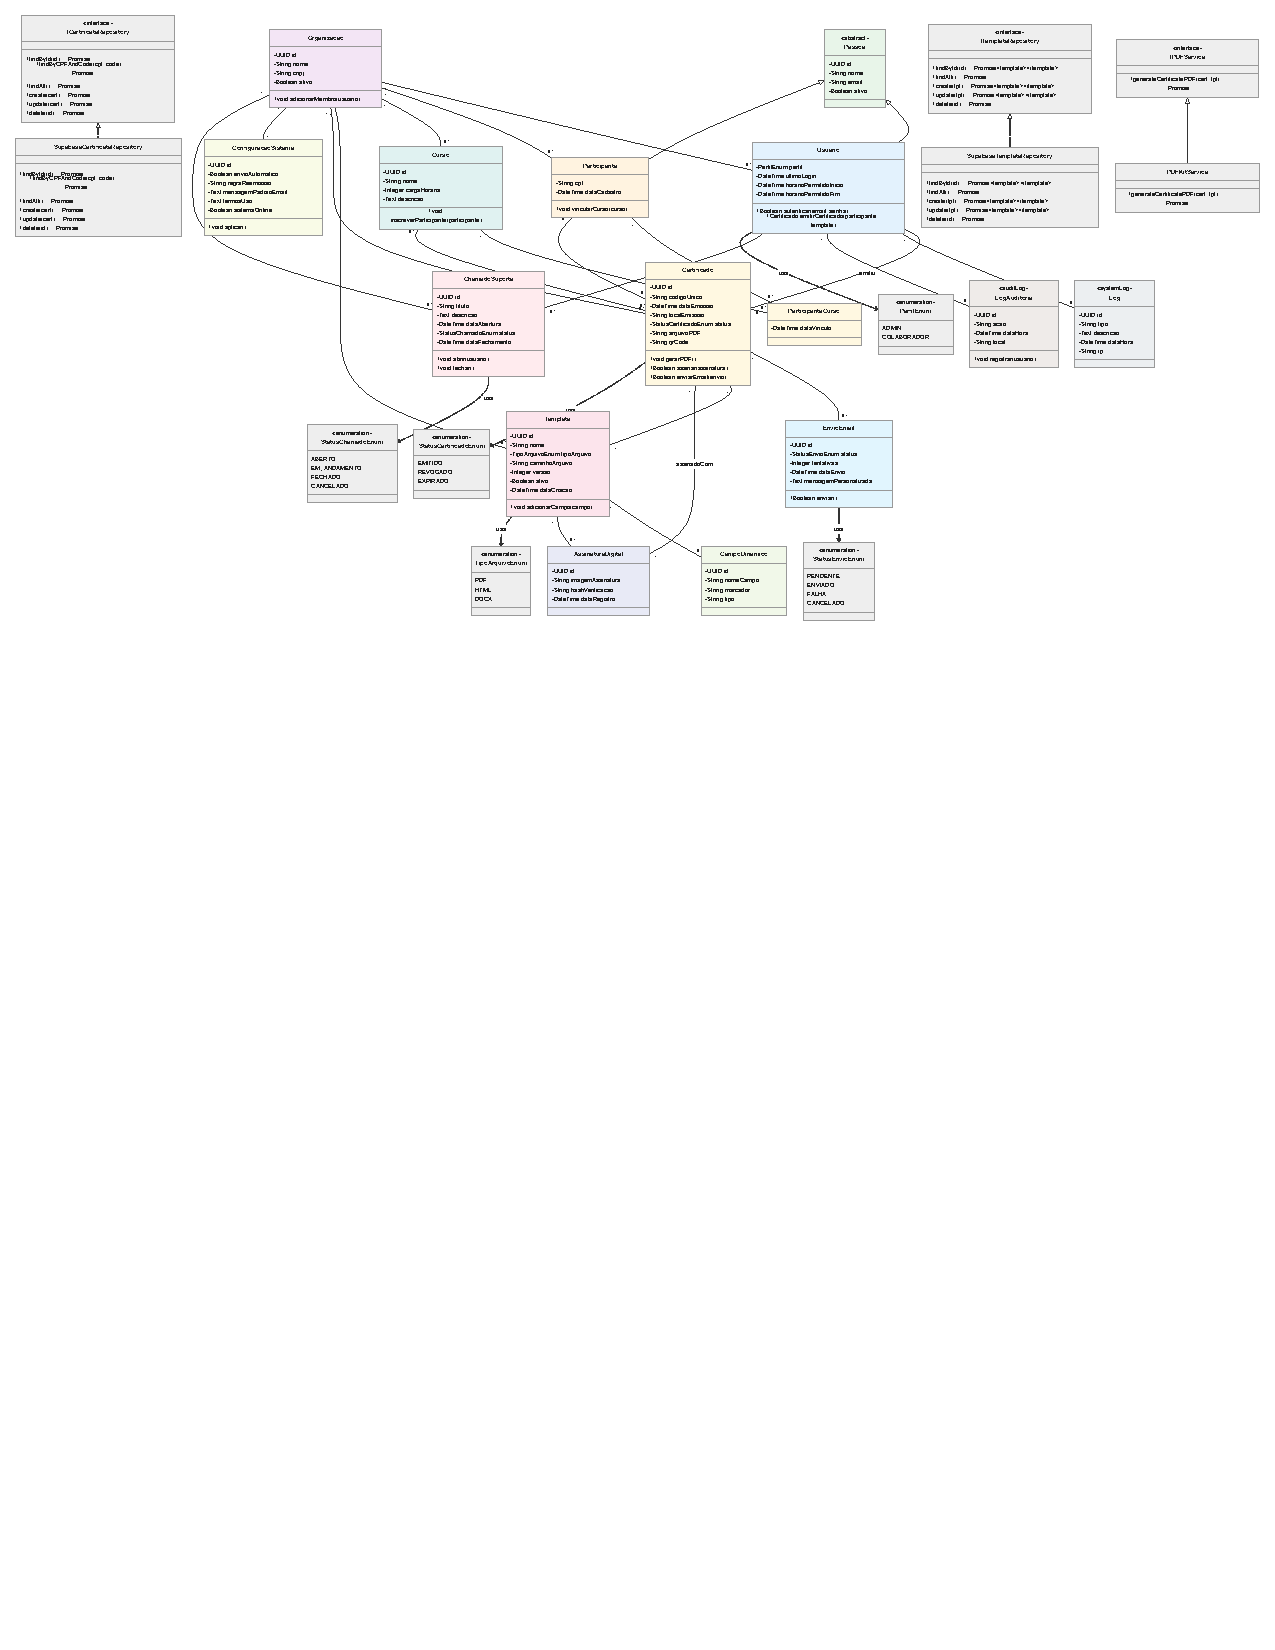
\includegraphics[width=0.9\textwidth]{imagens/diagrama-de-classes.pdf}
    \caption{Diagrama de Classes --- Sistema de Certificados}
    \label{fig:diagrama-classes}
\end{figure}



\subsection{Arquitetura do Sistema}

A arquitetura do sistema foi projetada para atender aos requisitos de independência entre camadas, testabilidade e facilidade de manutenção. Optou-se por uma abordagem de duas aplicações independentes --- frontend e backend --- que se comunicam exclusivamente via API REST. Essa separação permite que cada aplicação seja desenvolvida, testada, implantada e escalada de forma independente, sem acoplamento tecnológico entre as camadas de apresentação e lógica de negócio.

O backend adota uma arquitetura em quatro camadas, organizadas pelo princípio de inversão de dependências, em que camadas externas dependem de camadas internas:

\begin{enumerate}
    \item \textbf{Apresentação (\textit{App})} --- \textit{Route Handlers} do Next.js que expõem os endpoints REST (\code{/api/certificates}, \code{/api/templates}, \code{/api/verify}) e o utilitário \texttt{handle\-Api\-Error}, que converte exceções de domínio e erros de validação Zod em respostas HTTP padronizadas. Esta camada recebe a requisição, faz o \textit{parse} do JSON, aciona a validação do DTO e delega a execução ao \textit{use case}.
    \item \textbf{Aplicação (\textit{Application})} --- \textit{Use cases} que orquestram o fluxo de negócio (Emitir, Listar, Verificar, Gerar PDF, Gerenciar Templates) e \textbf{DTOs} definidos como esquemas Zod (\code{EmitCertificateDTO}, \code{UpdateValidityDTO}, \code{VerifyCertificateDTO}, etc.), que validam os dados de entrada antes de alcançarem o domínio.
    \item \textbf{Domínio (\textit{Domain})} --- Núcleo da aplicação, sem dependências externas. Contém as \textbf{entidades} (\code{Certificate}, \code{Template}) com suas regras de negócio encapsuladas, \textbf{interfaces de repositório} (\code{ICertificateRepository}, \code{ITemplateRepository}), \textbf{interfaces de serviço} (\code{IPDFService}), \textbf{\textit{Value Objects}} (\code{VerificationCode}, com geração e validação de código único) e \textbf{erros de domínio} (\code{CertificateNotFoundError}, \code{InvalidCertificateDataError}, etc.).
    \item \textbf{Infraestrutura (\textit{Infrastructure})} --- Implementações concretas das interfaces definidas no domínio: \code{SupabaseCertificateRepository}, \code{SupabaseTemplateRepository} e \code{PDFKitService}, além dos clientes de acesso ao banco PostgreSQL gerenciado pelo Supabase.
\end{enumerate}

O fluxo de dados percorre as camadas da seguinte forma: uma requisição HTTP chega ao \textit{Route Handler} (Apresentação), que valida o corpo da requisição contra o esquema Zod (Aplicação) e invoca o \textit{use case}. O \textit{use case} orquestra as operações de negócio utilizando entidades e \textit{Value Objects} do Domínio, e persiste os dados por meio das interfaces de repositório --- cujas implementações concretas (Infraestrutura) são injetadas via construtor. A resposta segue o caminho inverso até ser retornada ao cliente. Esse isolamento garante que as regras de negócio permaneçam independentes de frameworks, bancos de dados ou serviços externos. A inversão de dependência é obtida por meio de interfaces definidas no domínio e implementadas na infraestrutura --- por exemplo, \code{ICertificateRepository} e \code{IPDFService} são contratos que o \textit{use case} de emissão consome sem conhecer a implementação concreta. Entre as limitações desta abordagem, destaca-se o aumento do número de arquivos e interfaces, o que pode elevar a complexidade inicial do projeto em comparação com arquiteturas mais simples como \textit{controllers} monolíticos.

O frontend adota uma arquitetura em camadas com React, composta por quatro camadas que separam responsabilidades de forma clara. A \textbf{View} (apresentação) contém os componentes React que renderizam a interface do usuário, divididos em páginas (\code{views/}) e componentes reutilizáveis (\code{components/}), incluindo os do shadcn/ui. A \textbf{ViewModel} (lógica de apresentação) é formada por custom hooks (\code{useCertificatesViewModel}, \code{useDashboardViewModel}, etc.) que encapsulam estado (\code{useState}), efeitos colaterais (\code{useEffect}) e dados derivados (\code{useMemo}), expondo um objeto com estado e manipuladores para a camada View. O \textbf{Service} (infraestrutura) centraliza a comunicação com o backend: o módulo \code{api.ts} consome a API REST via \code{fetch}, e o módulo \code{envios.ts} gerencia a fila local de envios de e-mail no \code{localStorage} --- armazenando apenas dados operacionais (nome e e-mail do destinatário, \textit{status} da entrega), sem tokens de autenticação ou credenciais. O \textbf{Model} (domínio) reúne as interfaces TypeScript que definem as entidades do sistema (\code{Certificate}, \code{Template}, \code{VerifyResult}, \code{EnvioEmail}). O TanStack Router orquestra a navegação entre as Views, e o Tailwind CSS gerencia a estilização em todas as camadas de apresentação. Essa separação permite testar a lógica de apresentação independentemente da interface, utilizando Jest para validar os ViewModels sem depender de um navegador. Como limitação, o aumento do número de ViewModels eleva a quantidade de arquivos e hooks, o que pode tornar a navegação entre camadas mais custosa em projetos de grande escala.

O fluxo de comunicação entre as duas aplicações ocorre da seguinte forma: o frontend SPA, executado no navegador, faz requisições HTTPS aos \textit{Route Handlers} do backend por meio do módulo \code{api.ts} (camada Service), que encapsula a \code{fetch} API nativa. As requisições são autenticadas via token JWT gerenciado pelo Supabase Auth e trafegam sobre HTTPS (TLS 1.2), conforme RNF044. O backend processa a requisição através de suas quatro camadas --- Apresentação, Aplicação, Domínio e Infraestrutura --- e retorna a resposta padronizada ao frontend. Esse fluxo ponta a ponta está representado nos diagramas das Figuras~\ref{fig:backend} e~\ref{fig:frontend}, onde a seta "HTTPS REST + JWT" conecta o frontend SPA aos \textit{Route Handlers} do backend.

\begin{figure}[H]
    \centering
    \caption{Arquitetura do Backend — Quatro camadas (App, Application, Domain, Infrastructure) com DTOs, Value Objects e fluxo de dependências}
    \label{fig:backend}
    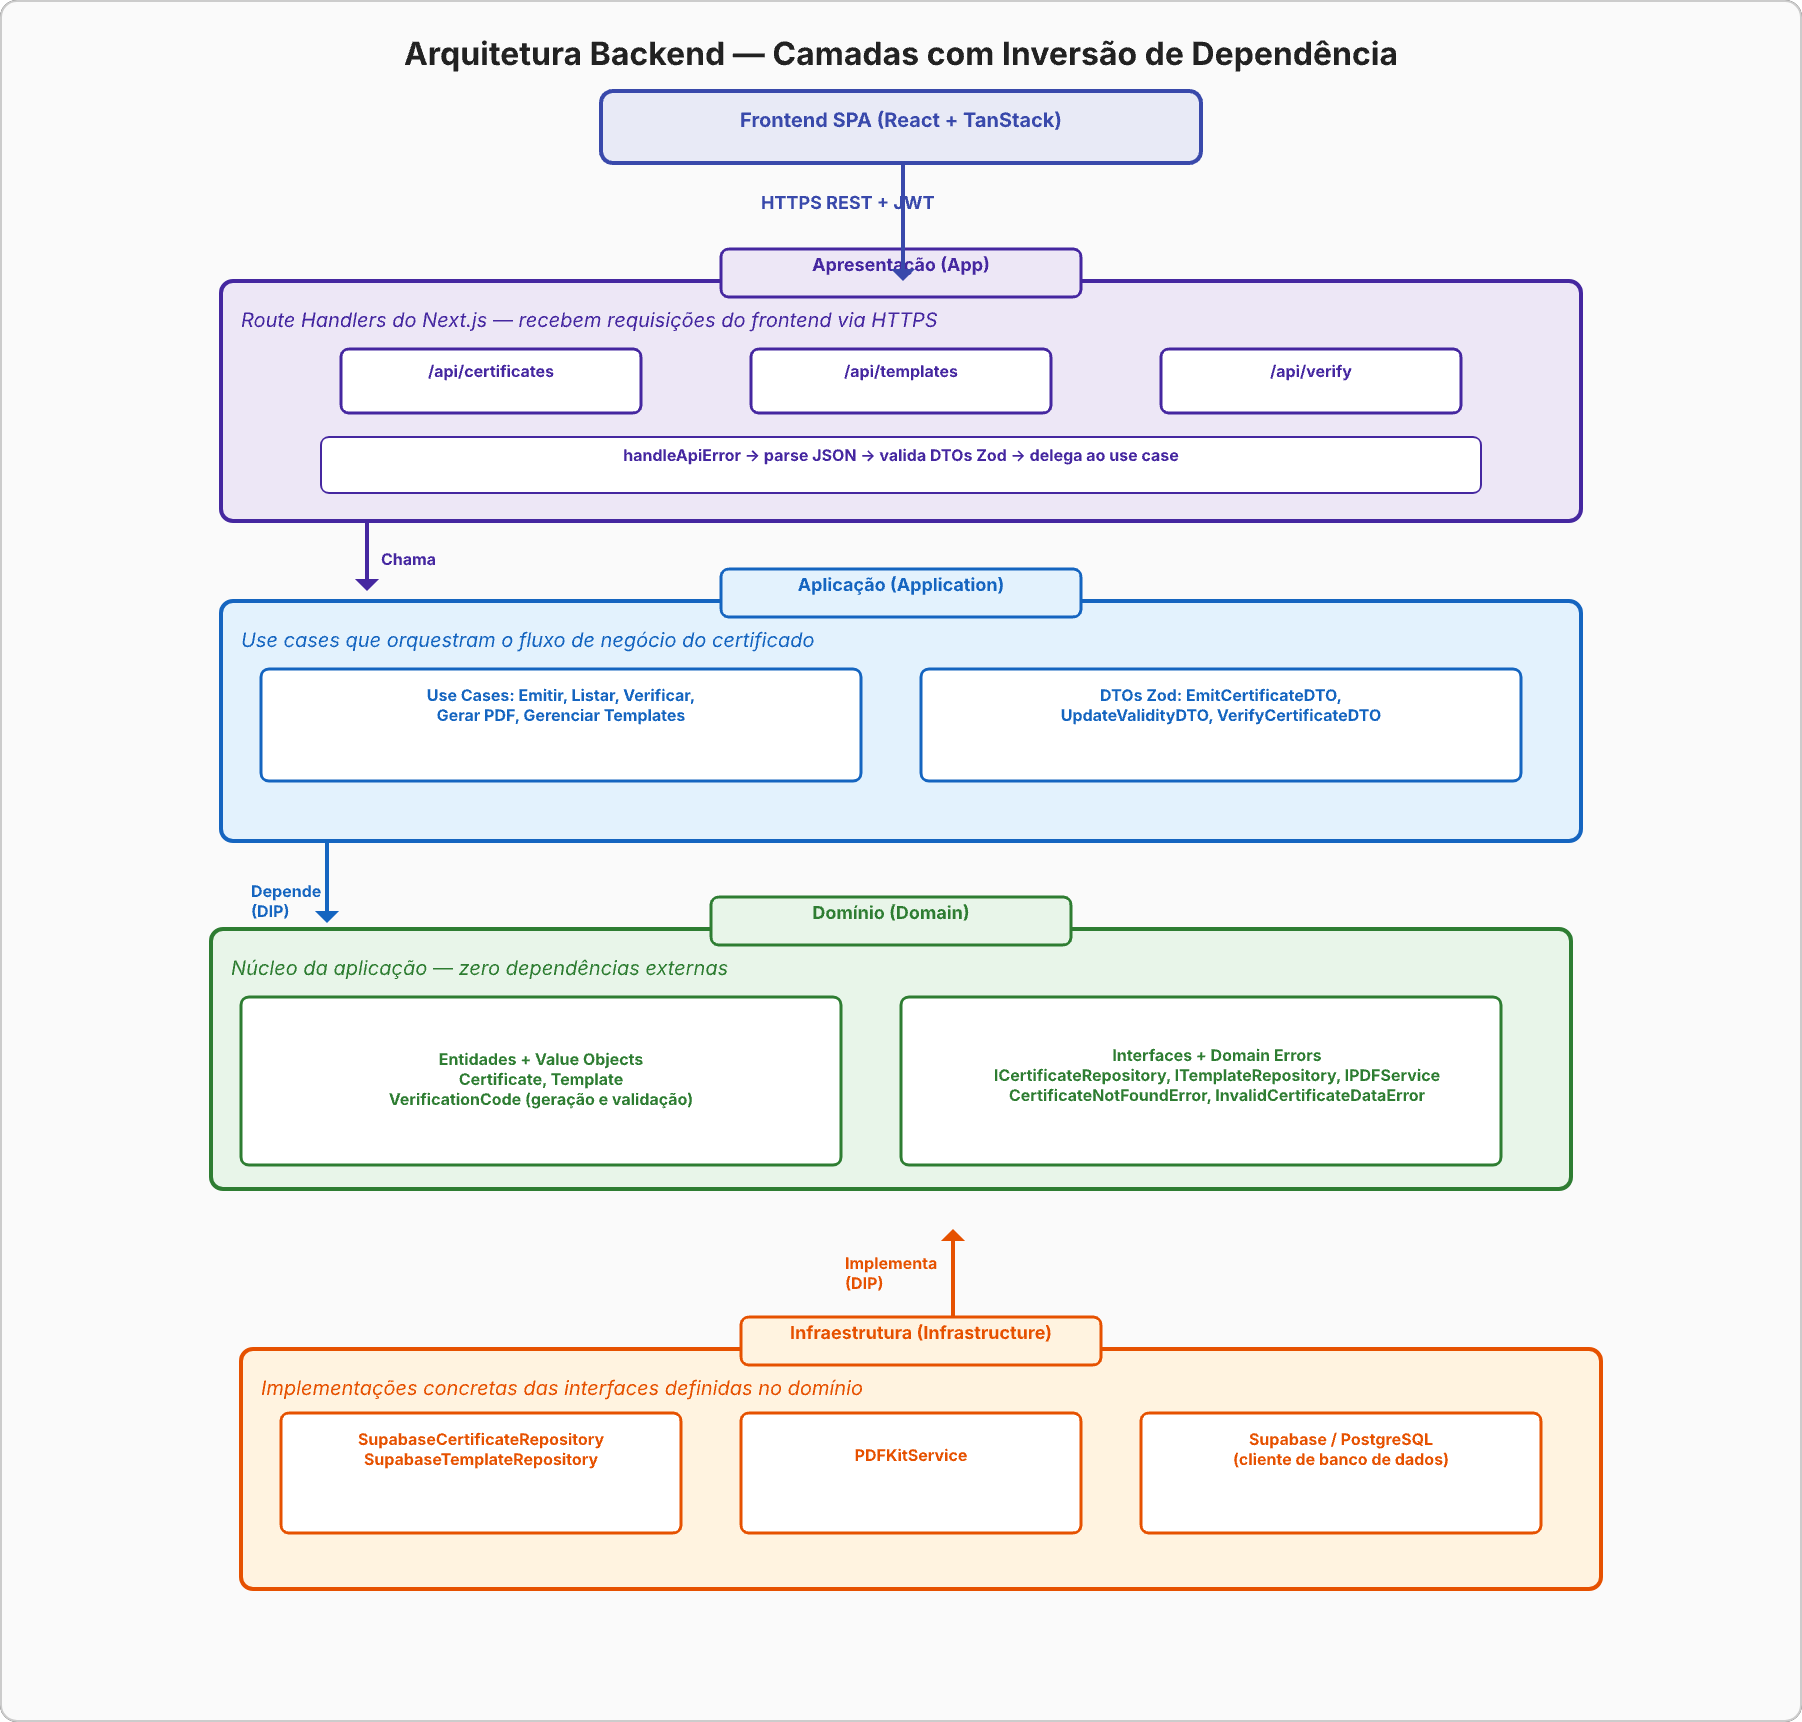
\includegraphics[width=0.9\textwidth]{imagens/backend.png}
    \par\vspace{0.5em}
    \parbox{\textwidth}{\raggedright\small\textit{Fonte: Elaborado pelo Autor (2026).}}
\end{figure}


\begin{figure}[H]
    \centering
    \caption{Arquitetura do Frontend — Quatro camadas (View, ViewModel, Service, Model) com React}
    \label{fig:frontend}
    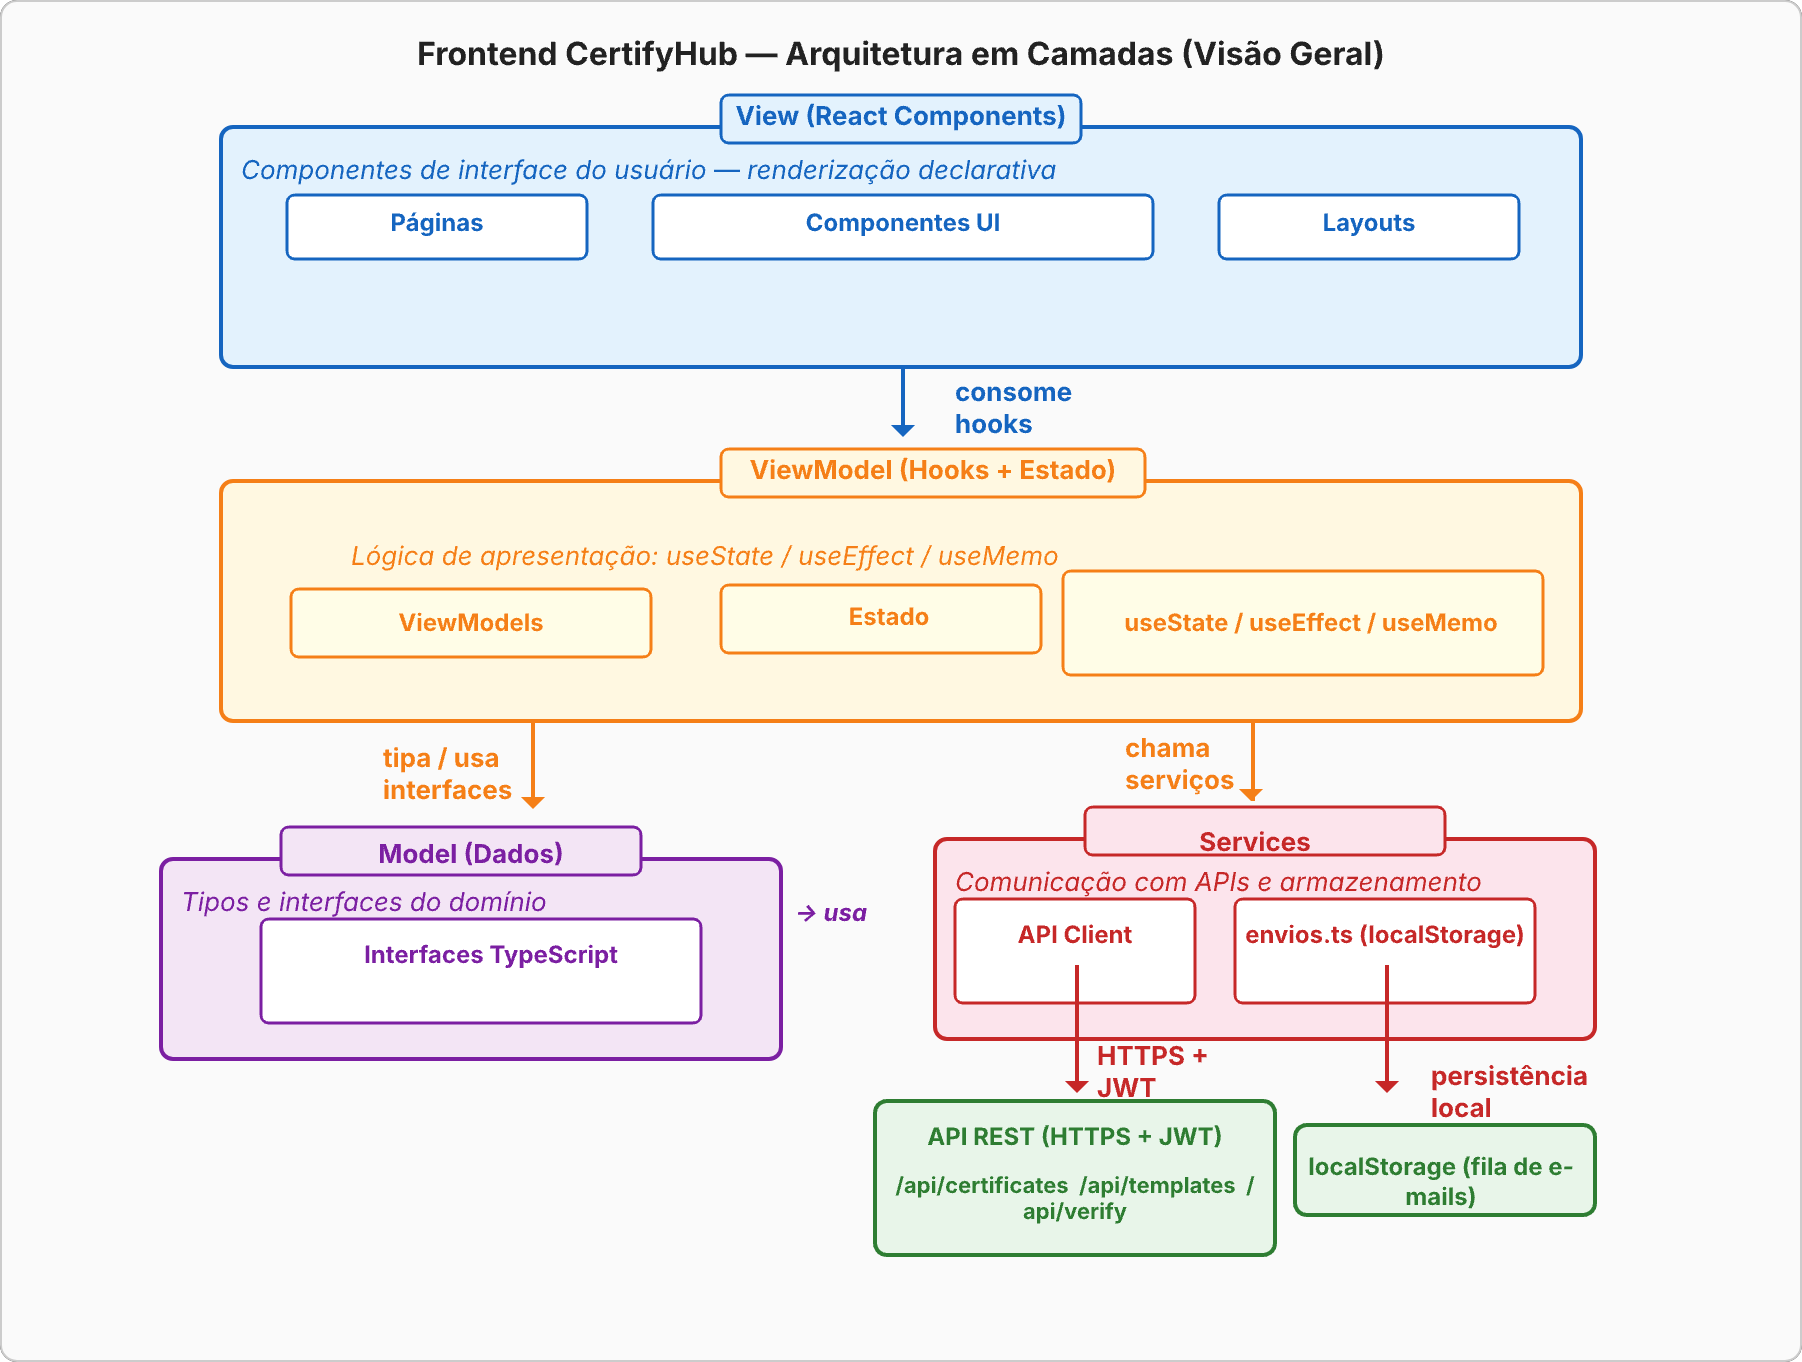
\includegraphics[width=0.9\textwidth]{imagens/frontend.png}
    \par\vspace{0.5em}
    \parbox{\textwidth}{\raggedright\small\textit{Fonte: Elaborado pelo Autor (2026).}}
\end{figure}


\subsection{Diagrama Entidade-Relacionamento}
O Diagrama Entidade-Relacionamento da Figura~\ref{fig:der} modela a estrutura do banco de dados implementada no MVP do sistema, composta por duas entidades principais: \code{CERTIFICADOS} e \code{TEMPLATES}. A notação adotada é a pé-de-galinha (Engenharia da Informação), onde o símbolo de barra (---) indica o lado ``1'' e o símbolo de três pontas (--<) indica o lado ``N'' (muitos). Ambas as entidades utilizam UUID como identificador primário.

A entidade \code{CERTIFICADOS} armazena os certificados emitidos e contém os seguintes atributos: \code{id} (PK, UUID), \code{recipientName} (varchar 200, NOT NULL), \code{recipientCPF} (varchar 11, NOT NULL, indexado), \code{courseName} (varchar 300, NOT NULL), \code{courseHours} (integer, NOT NULL), \code{verificationCode} (varchar 8, UNIQUE, NOT NULL), \code{validityDate} (timestamptz, NOT NULL), \code{templateId} (FK, UUID, NOT NULL), \code{issuedAt} (timestamptz, NOT NULL), \code{createdAt} (timestamptz, NOT NULL) e \code{updatedAt} (timestamptz, NOT NULL).

A entidade \code{TEMPLATES} gerencia os modelos de certificado disponíveis para emissão, com os atributos: \code{id} (PK, UUID), \code{name} (varchar 100, NOT NULL), \code{description} (text), \code{layoutConfig} (jsonb), \code{createdAt} (timestamptz, NOT NULL) e \code{updatedAt} (timestamptz, NOT NULL).

O relacionamento entre as entidades é de 1:N (um template pode ser usado por vários certificados), materializado pela chave estrangeira \code{templateId} na entidade \code{CERTIFICADOS} que referencia \code{TEMPLATES(id)}. Essa modelagem reflete o escopo reduzido do MVP, que contempla exclusivamente as funcionalidades de emissão de certificados com suporte a templates personalizáveis, sem as entidades de usuários, organizações, participantes, cursos e auditoria que serão incorporadas em versões futuras do sistema.

Vale ressaltar que, no estado atual do sistema, as informações relativas a participantes e cursos são armazenadas de forma denormalizada diretamente na entidade \code{CERTIFICADOS}, por meio dos atributos \code{recipientName}, \code{recipientCPF}, \code{courseName} e \code{courseHours}. Essa abordagem elimina a necessidade de chaves estrangeiras para entidades de participantes e cursos, simplificando a implementação do MVP, porém introduz redundância de dados e compromete a integridade referencial. Em versões futuras, as entidades \code{PARTICIPANTES} e \code{CURSOS} serão materializadas no banco de dados, permitindo a associação por meio de chaves estrangeiras (\code{participantId} e \code{courseId}), eliminando a duplicação de dados e habilitando funcionalidades como histórico de certificados por participante, listagem de certificados por curso e relatórios gerenciais por unidade de treinamento.

O Diagrama de Classes (Figura~\ref{fig:diagrama-classes}) apresenta a hierarquia \code{PESSOA} $\rightarrow$ \code{USUARIO} / \code{PARTICIPANTE} como uma generalização conceitual oriunda do modelo de domínio. No banco de dados físico do MVP, essas entidades não foram materializadas --- apenas \code{CERTIFICADOS} e \code{TEMPLATES} existem como tabelas. A implementação futura dessa herança seguirá a estratégia \textit{joined-table} (ou \textit{table-per-type}), na qual \code{PESSOA} seria uma tabela concreta com os atributos comuns (\code{id}, \code{nome}, \code{email}) e cada subtipo (\code{USUARIO}, \code{PARTICIPANTE}) teria sua própria tabela com chave primária que é também chave estrangeira referenciando \code{PESSOA(id)} --- garantindo integridade referencial sem armazenamento redundante.

\begin{figure}[H]
    \centering
    \caption{Diagrama Entidade-Relacionamento (DER) --- MVP do Banco de Dados}
    \label{fig:der}
    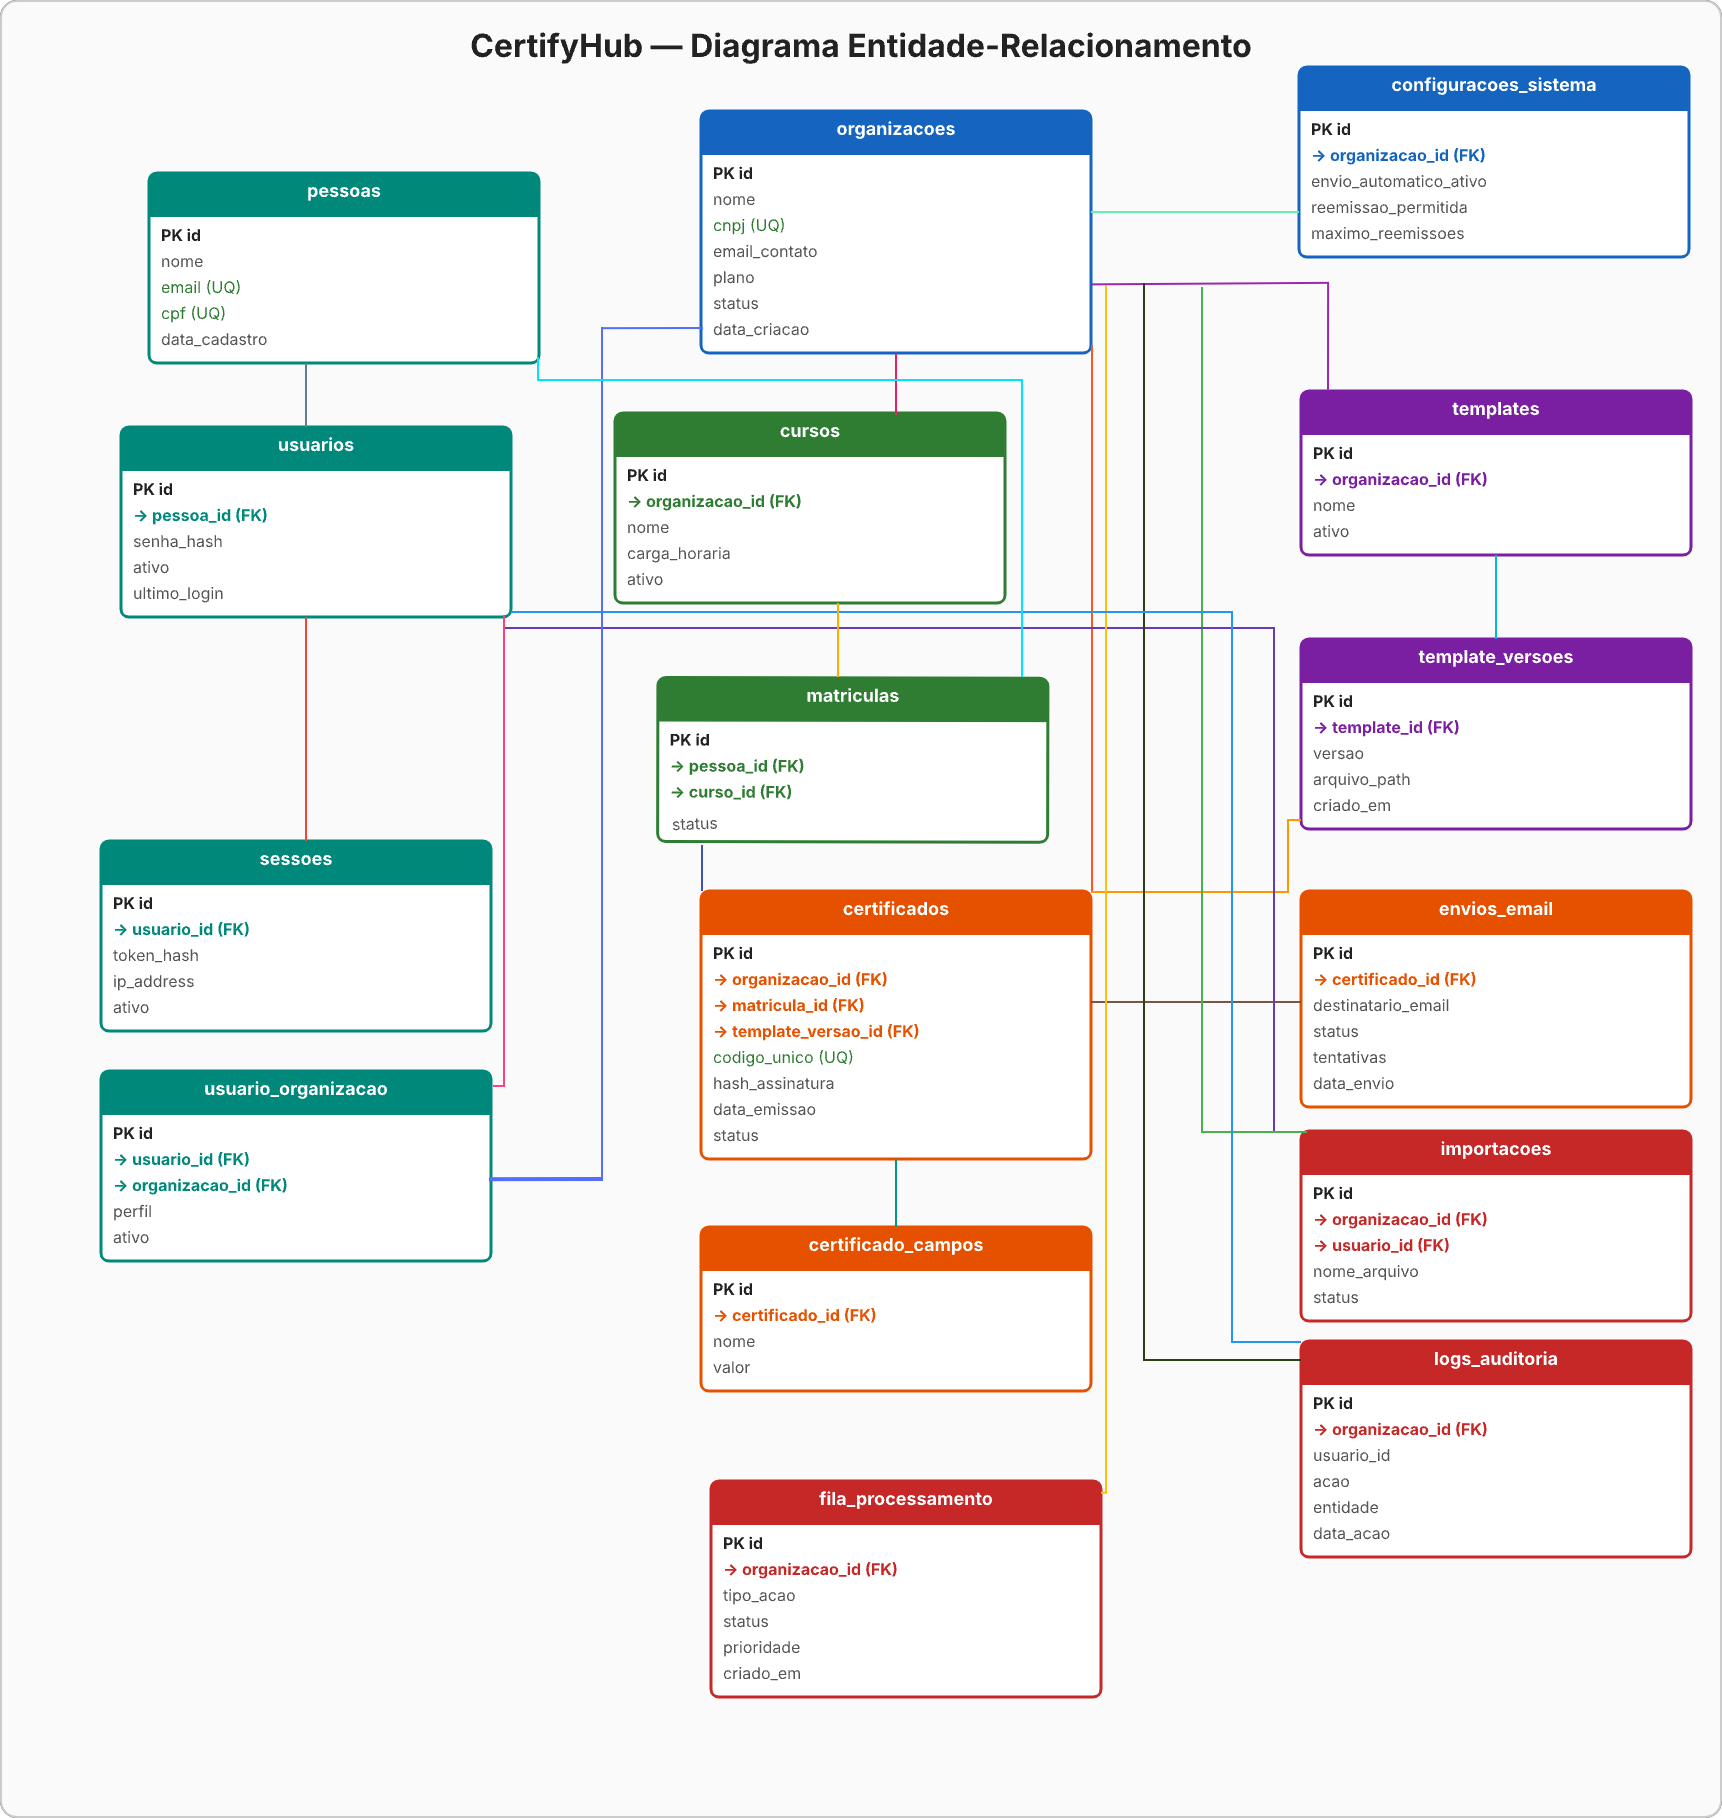
\includegraphics[width=0.9\textwidth]{imagens/DER.png}
\end{figure}

\subsection{Interfaces}
\begin{figure}[H]
    \centering
    
\includegraphics[width=\textwidth]{imagens/interface.png}
    \caption{Interface do Sistema --- Dashboard de Certificados}
    \label{fig:interface}
\end{figure}



% SOFTWARE
\section{SOFTWARE}

\subsection{Implantação}

O sistema é composto por duas aplicações independentes implantadas na plataforma Render, a partir de dois repositórios no GitHub: frontend (\url{https://github.com/igordev23/certificate-hub}) e backend (\url{https://github.com/igordev23/Certificate-server}). O sistema é publicado sob subdomínios automáticos fornecidos pela plataforma, garantindo tráfego criptografado via SSL/HTTPS de forma nativa. O frontend pode ser acessado, por exemplo, em \url{https://certificate-hub.onrender.com}, enquanto a API do backend responde em \url{https://certificate-server-zd0m.onrender.com}.

\subsubsection{Arquitetura e Execução}

Para a execução e construção do projeto, é estipulado o uso do Node.js, configurado no Render através da variável de ambiente \texttt{NODE\_VERSION}. A implantação distingue a arquitetura das duas aplicações:

\begin{itemize}
    \item \textbf{Frontend (Static Site):} Trata-se de uma \textit{Single Page Application} (SPA) em Vite. O serviço de \textit{Static Site} serve exclusivamente arquivos estáticos (HTML, CSS e JavaScript gerados na pasta \texttt{dist}) diretamente, sem manter um processo de execução ativo (\textit{runtime} Node). O roteamento no lado do cliente é delegado ao TanStack Router via \textit{History API}.
    \item \textbf{Backend (Web Service):} Construído em Next.js (utilizando recursos de servidor Node.js), opera como um \textit{Web Service}, ou seja, mantém um processo vivo que processa requisições HTTP dinâmicas em tempo real. O processo de implantação exige a execução do comando de compilação (\texttt{npm run build}) antes da inicialização do servidor com \texttt{npm start}.
\end{itemize}

\subsubsection{CI/CD e Pipeline de Implantação}

O fluxo de implantação baseia-se em um pipeline de CI/CD (Integração e Entrega Contínuas). A etapa de \textit{Continuous Integration} (CI) é gerenciada pelo GitHub Actions, que executa automaticamente as suítes de testes a cada \textit{push} na branch \texttt{main}. Se os testes passarem com sucesso, a etapa de \textit{Continuous Deployment} (CD) é acionada no Render, que compila e publica a nova versão. Em caso de falha nos testes (no GitHub Actions) ou no \textit{build} (no Render), o processo é interrompido, impedindo que código defeituoso chegue a produção. Caso um comportamento inesperado ocorra pós-deploy, a plataforma fornece uma estratégia simples de \textit{rollback}, permitindo reverter imediatamente para o \textit{deploy} anterior funcional com um único clique. A Figura~\ref{fig:deploy} ilustra o fluxo.

\begin{figure}[H]
\centering
\caption{Pipeline de CI do backend no GitHub Actions}
\label{fig:ci-backend}
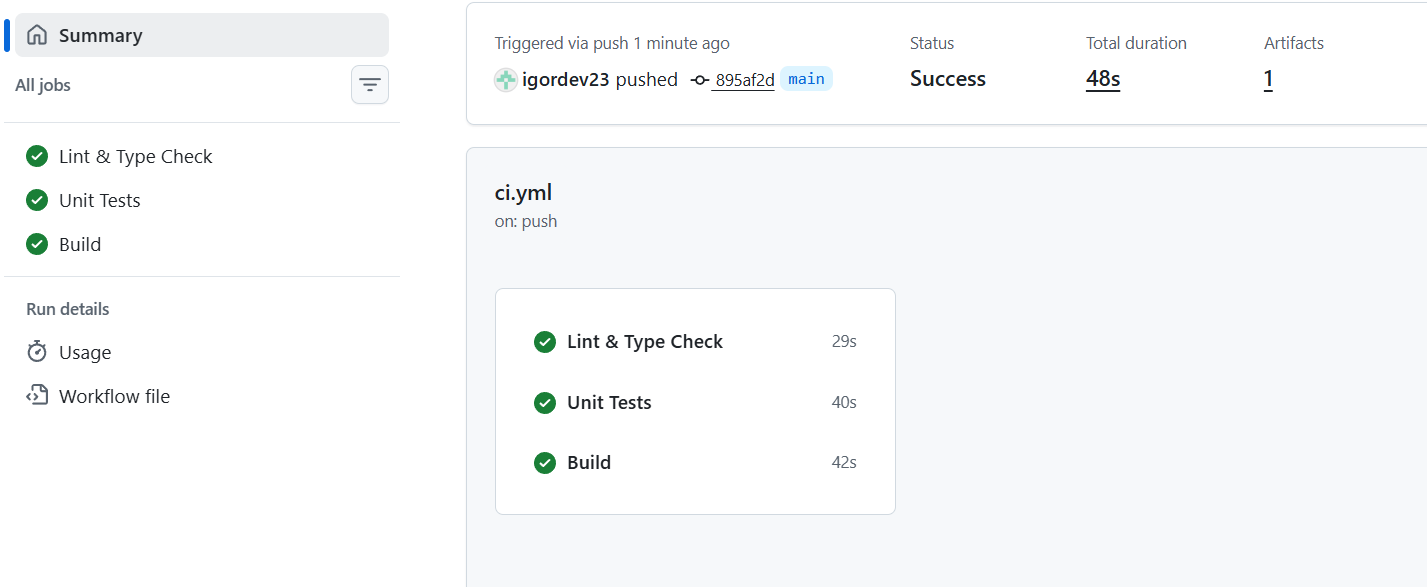
\includegraphics[width=\textwidth]{imagens/CIbackend.png}
\par\vspace{0.5em}
\parbox{\textwidth}{\raggedright\small\textit{Fonte: Elaborado pelo Autor (2026).}}
\end{figure}

\begin{figure}[H]
\centering
\caption{Pipeline de CI do frontend no GitHub Actions}
\label{fig:ci-frontend}
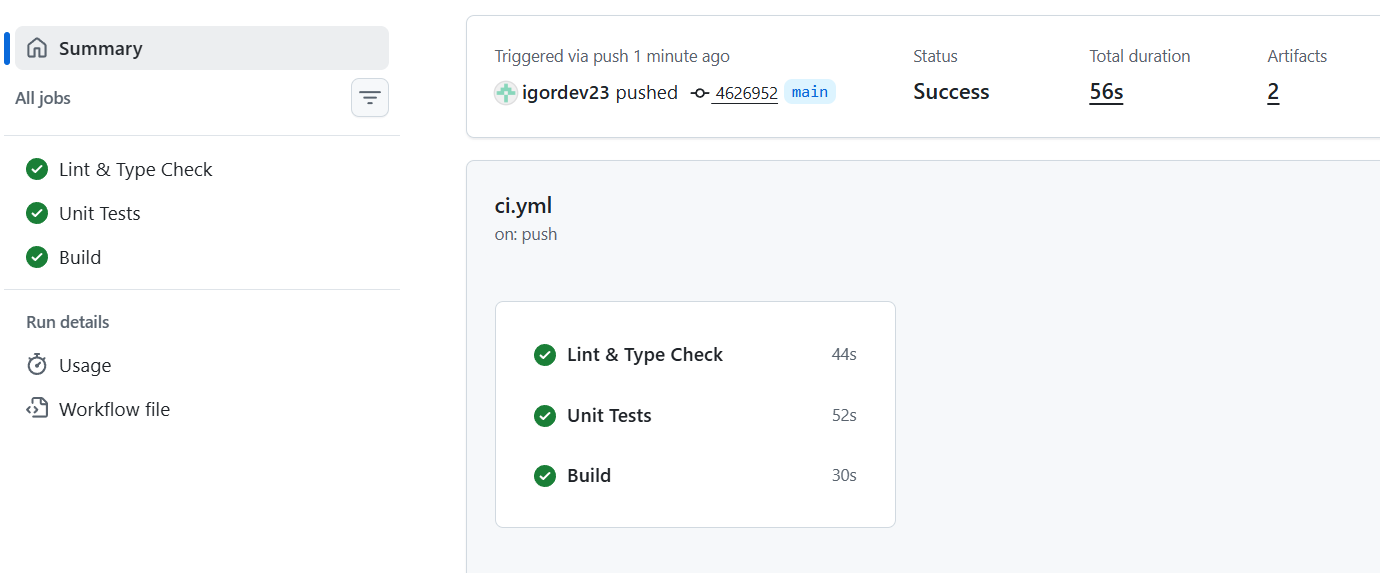
\includegraphics[width=\textwidth]{imagens/CIfrontend.png}
\par\vspace{0.5em}
\parbox{\textwidth}{\raggedright\small\textit{Fonte: Elaborado pelo Autor (2026).}}
\end{figure}

\subsubsection{Configuração de Ambiente}

Para assegurar o isolamento das configurações sensíveis, utilizam-se variáveis de ambiente não expostas no código. Os modelos de configuração adotados incluem:

\begin{itemize}
    \item \textbf{Frontend:} \texttt{VITE\_API\_URL} (aponta para a URL do Web Service backend).
    \item \textbf{Backend:}
    \begin{itemize}
        \item \texttt{DATABASE\_URL} (string de conexão PostgreSQL);
        \item \texttt{NEXT\_PUBLIC\_SUPABASE\_URL} (URL do projeto Supabase);
        \item \texttt{NEXT\_PUBLIC\_SUPABASE\_PUBLISHABLE\_KEY} (chave pública do Supabase);
        \item \texttt{NEXT\_PUBLIC\_FRONTEND\_URL} (URL do frontend para configuração de CORS).
    \end{itemize}
\end{itemize}

\subsubsection{Banco de Dados}

O armazenamento é delegado ao PostgreSQL hospedado via Supabase. O banco de dados utiliza \textit{connection pooling} nativo (gerenciamento de conexões otimizado) para alta concorrência e conta com política de backup automático gerida pela plataforma. As atualizações estruturais (\textit{schema}) são aplicadas através de migrações executadas automaticamente na fase de \textit{build}.

\subsubsection{Monitoramento e Observabilidade}

Por fim, a observabilidade do sistema e o monitoramento (\textit{health checks}) são garantidos pelos logs em tempo real nativos do Render, permitindo diagnóstico ágil de eventuais gargalos de desempenho e verificação de saúde da aplicação.

\begin{figure}[H]
    \centering
    \caption{Diagrama de Implantação — Fluxo de deploy no Render a partir do GitHub, com frontend como Static Site, backend como Web Service e banco PostgreSQL gerenciado pelo Supabase}
    \label{fig:deploy}
    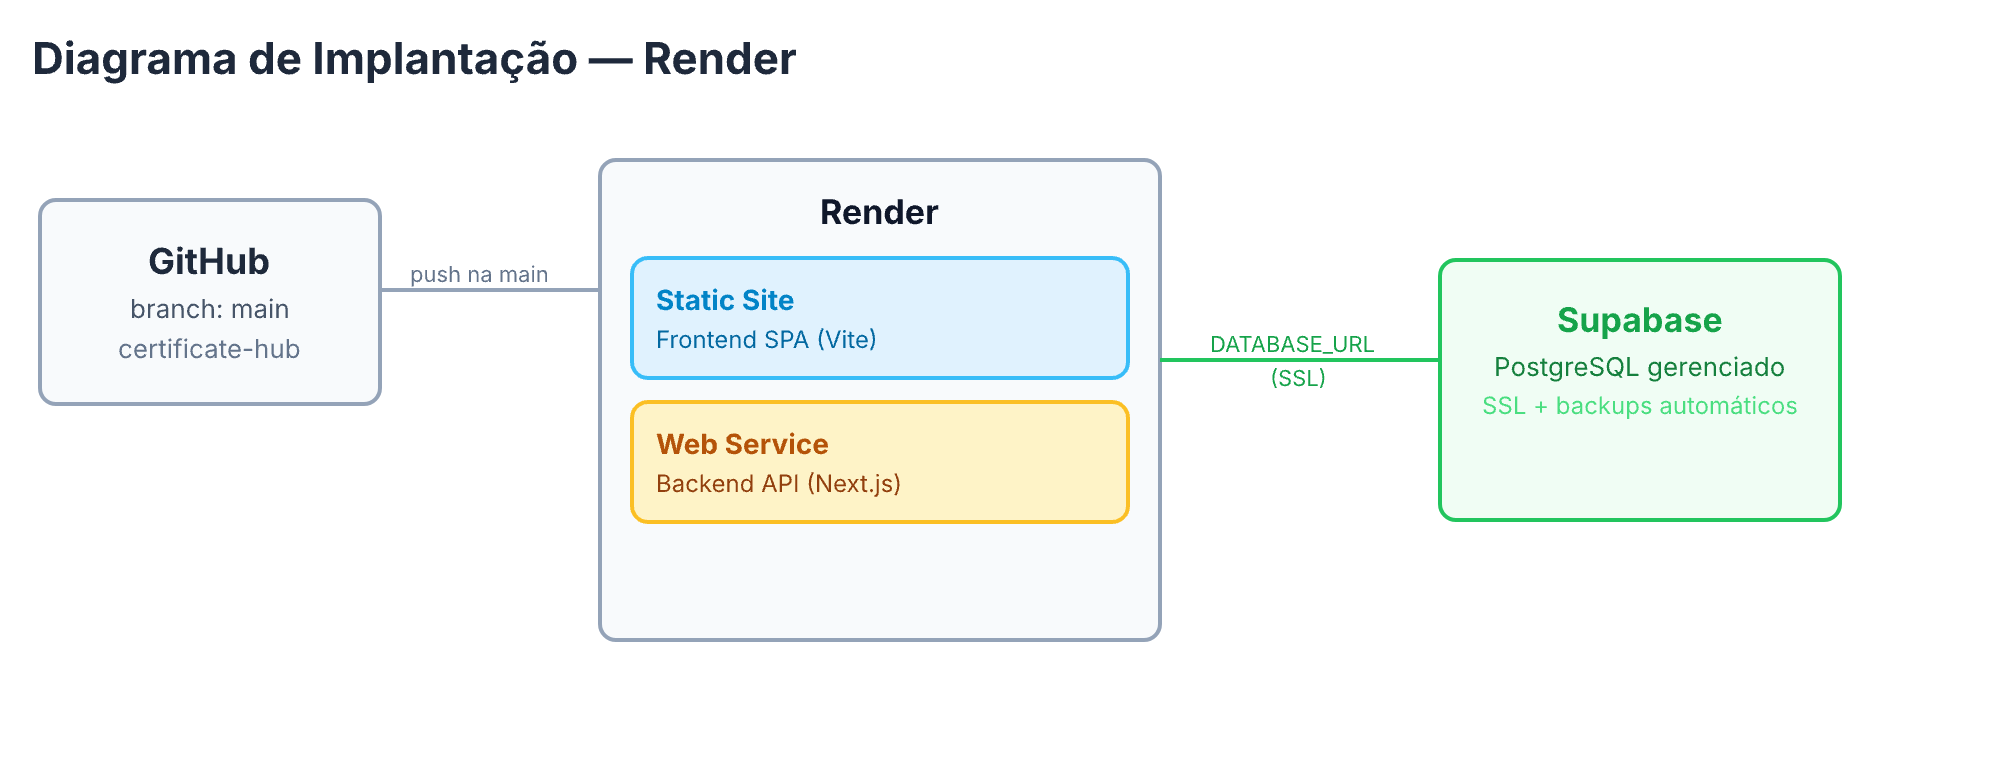
\includegraphics[width=0.85\textwidth]{imagens/deploy.png}
    \par\vspace{0.5em}
    \parbox{\textwidth}{\raggedright\small\textit{Fonte: Elaborado pelo Autor (2026).}}
\end{figure}


\subsection{Exemplos de Código}
\label{sec:exemplos-codigo}

Esta seção apresenta trechos reais do código-fonte do sistema que ilustram as principais funcionalidades implementadas. Os exemplos foram extraídos do backend (CertifyHub Server), construído com Next.js e TypeScript seguindo os princípios de arquitetura limpa.

\subsubsection{Entidade de Domínio: Certificate}
\label{sec:codigo-certificate}

O Código~\ref{cod:certificate} apresenta a entidade \code{Certificate}, que encapsula as regras de negócio relacionadas à emissão e validação de certificados. A classe utiliza um construtor privado e métodos estáticos de fábrica (\code{create} e \code{fromPersistence}) para garantir que apenas instâncias válidas sejam criadas. O método \code{isValid()} (linha~\ref{line:isvalid}) implementa a regra de negócio que determina se um certificado está dentro do prazo de validade, comparando a data de validade com a data atual.

\begin{lstlisting}[language=TypeScript, caption={Entidade Certificate com validações de domínio}, label={cod:certificate}, escapechar=§]
export class Certificate {
  private constructor(private props: CertificateProps) {}

  static create(props: Omit<CertificateProps, "createdAt" | "updatedAt">): Certificate {
    Certificate.validate(props);
    return new Certificate({ ...props, createdAt: new Date(), updatedAt: new Date() });
  }

  static fromPersistence(props: CertificateProps): Certificate {
    return new Certificate({ ...props, validityDate: new Date(props.validityDate) });
  }

  isValid(): boolean {       §\label{line:isvalid}§
    return this.props.validityDate > new Date();
  }

  updateValidity(newDate: Date): void {
    if (newDate <= new Date()) throw new InvalidValidityDateError();
    this.props.validityDate = newDate;
    this.props.updatedAt = new Date();
  }

  private static validate(props: Omit<CertificateProps, "createdAt" | "updatedAt">): void {
    if (!props.recipientName?.trim()) throw new InvalidCertificateDataError("Nome é obrigatório");
    if (!props.recipientCPF || props.recipientCPF.length !== 11)
      throw new InvalidCertificateDataError("CPF deve ter 11 dígitos");
    if (!props.courseHours || props.courseHours <= 0)
      throw new InvalidCertificateDataError("Carga horária deve ser maior que zero");
    if (!props.templateId) throw new InvalidCertificateDataError("Template é obrigatório");
  }
}
\end{lstlisting}
\noindent\raggedright\small\textit{Fonte: Elaborado pelo Autor (2026).}

\subsubsection{Route Handler de Emissão}
\label{sec:codigo-emissao}

O Código~\ref{cod:emit} mostra o \textit{Route Handler} responsável pela emissão de certificados (\ref{rf:gerar-pdf}). A requisição \code{POST /api/certificates/emit} recebe os dados do certificado, valida-os com Zod (\code{emitCertificateSchema.parse}), instancia os repositórios concretos e delega a execução ao caso de uso \code{EmitCertificateUseCase}. O uso de injeção de dependência nos repositórios (linhas~\ref{line:repos} e~\ref{line:repos2}) permite substituir as implementações sem alterar a lógica de negócio.

\begin{lstlisting}[language=TypeScript, caption={Route Handler de emissão de certificado}, label={cod:emit}, escapechar=§]
export async function POST(request: Request) {
  try {
    const body = await request.json();
    const validated = emitCertificateSchema.parse(body);

    const certificateRepo = new SupabaseCertificateRepository();§\label{line:repos}§
    const templateRepo = new SupabaseTemplateRepository();§\label{line:repos2}§
    const useCase = new EmitCertificateUseCase(certificateRepo, templateRepo);

    const { certificate } = await useCase.execute(validated);

    return NextResponse.json(
      { data: certificate.toJSON(), message: "Certificado emitido com sucesso" },
      { status: 201 }
    );
  } catch (error) {
    return handleApiError(error);
  }
}
\end{lstlisting}
\noindent\raggedright\small\textit{Fonte: Elaborado pelo Autor (2026).}

\subsubsection{Geração de PDF com \textit{QR Code}}
\label{sec:codigo-pdf}

O Código~\ref{cod:pdf} apresenta o serviço \code{PDFKitService} que gera o PDF do certificado com \textit{QR Code} de verificação (\ref{rf:qrcode}). A URL de verificação é montada a partir da variável de ambiente \code{NEXT\_PUBLIC\_VERIFY\_URL} (linha~\ref{line:verifyurl}) e codificada em um \textit{QR Code} utilizando a biblioteca \code{qrcode} (linha~\ref{line:qrcode}). A imagem gerada é inserida no PDF na posição inferior esquerda (linha~\ref{line:qrimage}), acompanhada das instruções de verificação e do código único.

\begin{lstlisting}[language=TypeScript, caption={Geração de PDF com QR Code no servidor}, label={cod:pdf}, escapechar=§]
const verifyUrl = `${process.env.NEXT_PUBLIC_VERIFY_URL ||§\label{line:verifyurl}§
  "https://example.com/verify"}?cpf=${certificate.recipientCPF}
  &codigo=${certificate.verificationCode}`;

const qrBuffer = await toBuffer(verifyUrl, {           §\label{line:qrcode}§
  width: 160, margin: 1,
  color: { dark: template.layoutConfig.primaryColor, light: "#ffffff" },
});

const doc = new PDFDocument({ layout: "landscape", size: "A4" });

// Posicionar QR Code no canto inferior esquerdo
doc.image(qrBuffer, 80, instrY, { width: 60 });        §\label{line:qrimage}§

// Instruções de verificação ao lado do QR Code
doc.font("Helvetica-Bold").fontSize(9).text(
  "INSTRUÇÕES PARA VERIFICAÇÃO DE AUTENTICIDADE:", instrX, instrY
);
doc.font("Helvetica").fontSize(8).text(
  \`Este certificado foi emitido pelo CertifyHub.
  Verifique a sua autenticidade acessando o QR Code...\`, instrX, instrY + 14
);
\end{lstlisting}
\noindent\raggedright\small\textit{Fonte: Elaborado pelo Autor (2026).}

\subsubsection{Validação por Código Único}
\label{sec:codigo-validacao}

O Código~\ref{cod:verify-handler} apresenta o \textit{Route Handler} público \code{POST /api/verify} que implementa a validação de autenticidade de certificados (\ref{rf:portal-validacao}--\ref{rf:exibir-validacao}). A requisição recebe o CPF e o código de verificação presentes no certificado, valida a entrada com Zod (\code{verifyCertificateSchema}) e delega a lógica ao \code{VerifyCertificateUseCase}.

\begin{lstlisting}[language=TypeScript, caption={Route Handler público de verificação de autenticidade}, label={cod:verify-handler}, escapechar=§]
export async function POST(request: Request) {
  try {
    const body = await request.json();
    const validated = verifyCertificateSchema.parse(body);

    const repo = new SupabaseCertificateRepository();
    const useCase = new VerifyCertificateUseCase(repo);
    const result = await useCase.execute(validated);

    return NextResponse.json({ data: result });
  } catch (error) {
    return handleApiError(error);
  }
}
\end{lstlisting}
\noindent\raggedright\small\textit{Fonte: Elaborado pelo Autor (2026).}

O Código~\ref{cod:verify-usecase} detalha o caso de uso \code{VerifyCertificateUseCase}, que centraliza a lógica de verificação. O método \code{execute} busca o certificado no banco por CPF e código (\ref{rf:validar-certificado}); se encontrado, retorna os dados do certificado e o status de validade calculado pelo método \code{isValid()} da entidade de domínio. Se não encontrado, indica que o certificado não é autêntico.

\begin{lstlisting}[language=TypeScript, caption={Caso de uso de verificação de autenticidade}, label={cod:verify-usecase}, escapechar=§]
export class VerifyCertificateUseCase {
  constructor(private readonly certificateRepo: ICertificateRepository) {}

  async execute(dto: VerifyCertificateDTO): Promise<VerifyCertificateResult> {
    const certificate = await this.certificateRepo.findByCPFAndCode(
      dto.cpf,
      dto.verificationCode.toUpperCase()
    );

    if (!certificate) {
      return { isAuthentic: false, isValid: false, certificate: null };
    }

    return {
      isAuthentic: true,
      isValid: certificate.isValid(),
      certificate: {
        recipientName: certificate.recipientName,
        courseName: certificate.courseName,
        courseHours: certificate.courseHours,
        issuedAt: certificate.issuedAt,
        validityDate: certificate.validityDate,
        verificationCode: certificate.verificationCode,
      },
    };
  }
}
\end{lstlisting}
\noindent\raggedright\small\textit{Fonte: Elaborado pelo Autor (2026).}

\subsection{Testes}

Conforme definido nos objetivos específicos da Seção~\ref{sec:objetivos-especificos}, foram planejados e executados testes unitários para validação dos módulos implementados no escopo do MVP. Os casos de teste foram elaborados com base nos critérios de aceitação apresentados no Quadro~\ref{qua:criterios} e abrangem os requisitos funcionais classificados como prioritários — \textit{Must have} [M] e \textit{Should have} [S] — essenciais para a primeira versão do sistema.

Os testes foram classificados como unitários, uma vez que cada módulo (frontend e backend) foi testado de forma isolada, com dependências externas (banco de dados, APIs de terceiros, bibliotecas de geração de PDF) substituídas por \textit{mocks}. Testes não-funcionais de carga, segurança (\textit{rate limiting} e autenticação) e acessibilidade foram implementados com escopo reduzido, conforme detalhado nas subseções seguintes. Testes de integração não foram incluídos no escopo do MVP, podendo ser abordados em versões futuras do sistema. Testes \textit{end-to-end} (E2E) foram implementados com Playwright para validar o fluxo completo do sistema, conforme descrito na Seção~\ref{subsubsec:e2e}. Todos os testes foram executados em ambiente local, com Node.js 22, e integraram o pipeline de CI/CD do Render, que executa a suíte completa a cada \textit{push} na branch \texttt{main}.

\subsubsection{Plano de Testes}

\paragraph{Estratégia de Testes}

O plano de testes foi elaborado com base nos requisitos funcionais (Seção~3.1.1) e nos critérios de aceitação (Quadro~\ref{qua:criterios}), contemplando exclusivamente os módulos implementados no escopo do MVP. A estratégia adotada prioriza testes unitários como primeira camada de defesa, combinada com testes de integração para validação das camadas de infraestrutura e testes \textit{end-to-end} (E2E) para verificação do fluxo completo do sistema.

\begin{itemize}
    \item \textbf{Ferramentas:} Jest como \textit{test runner} e \textit{framework} de asserção; React Testing Library para testes de \textit{ViewModels} no frontend; Playwright para testes \textit{end-to-end}; \textit{Mocking} manual via \texttt{jest.mock} para isolar dependências externas (Supabase, PDFKit, \texttt{fetch}).
    \item \textbf{Execução em CI/CD:} A suíte completa é executada automaticamente pelo Render a cada \textit{push} na branch \texttt{main}. O pipeline valida que todos os testes passem antes da implantação.
    \item \textbf{Meta de cobertura:} O projeto define cobertura mínima de 75\% em \textit{Statements}, \textit{Functions} e \textit{Lines}, configurada no Jest e validada no pipeline de CI. As camadas de domínio e casos de uso no backend têm meta informal de 100\%.
    \item \textbf{Massa de dados:} Os testes de repositório utilizam o cliente Supabase \textit{mockado}, dispensando banco de dados real. Para testes das entidades de domínio, os dados são construídos em memória (\textit{in-memory}), garantindo isolamento total entre cenários.
\end{itemize}

\paragraph{Casos de Teste}

Cada caso de teste é identificado por um código único (CT\textit{nnn}) e descreve o cenário avaliado juntamente com o resultado esperado. O Quadro~\ref{qua:plano-testes} apresenta o plano completo, organizado por módulo e tipo de teste.

\renewcommand{\arraystretch}{0.85}
\small
\begingroup
\renewcommand{\tablename}{Quadro}
\renewcommand{\LTcaptype}{quadro}
\begin{longtable}{p{1.2cm} p{4.2cm} p{7.5cm} p{2.6cm}}
\caption{Plano de testes do sistema}
\label{qua:plano-testes}\\
\toprule
\textbf{Caso} & \textbf{Descrição} & \textbf{Resultados Esperados} & \textbf{Status} \\
\midrule
\endfirsthead
\toprule
\textbf{Caso} & \textbf{Descrição} & \textbf{Resultados Esperados} & \textbf{Status} \\
\midrule
\endhead
\bottomrule
\endfoot
\bottomrule
\endlastfoot

\multicolumn{4}{l}{\textbf{Módulo de Templates de Certificados (\ref{rf:upload-templates}--\ref{rf:duplicar-templates})}} \\
\midrule

CT001 & Criação de template & Template é criado com nome, descrição e \textit{layout} mesclado aos valores padrão. & Executado \\
CT002 & Listagem de templates & \textit{Endpoint} retorna lista de templates cadastrados. & Executado \\
CT003 & Obtenção de template por ID & \textit{Endpoint} retorna template específico; lança erro \texttt{TemplateNotFoundError} se não existir. & Executado \\
CT004 & Edição de template & Nome, descrição e configurações de \textit{layout} são alterados e persistem. & Executado \\
CT005 & Exclusão de template & Template é removido após confirmação do usuário; \textit{endpoint} \texttt{delete} é chamado. & Executado \\
CT006 & Personalização de \textit{layout} & Configurações parciais são mescladas com os valores padrão (\texttt{DEFAULT\_LAYOUT}). & Executado \\

\midrule
\multicolumn{4}{l}{\textbf{Módulo de Geração de Certificados (\ref{rf:gerar-pdf}--\ref{rf:download-lote})}} \\
\midrule

CT007 & Emissão manual de certificado & Selecionar template, preencher dados e confirmar gera certificado com código único. & Executado \\
CT008 & Geração de PDF & PDF gerado preserva layout, cores e fontes do template; resultado é um \textit{Buffer} binário. & Executado \\
CT009 & Geração de PDF com cores personalizadas & PDF é gerado com \texttt{backgroundColor}, \texttt{primaryColor} e \texttt{borderColor} personalizados. & Executado \\
CT010 & Geração de PDF sem borda & PDF é gerado corretamente com \texttt{showBorder = false}. & Executado \\
CT011 & Erro na geração de PDF & Falha no PDFKit rejeita a \textit{Promise} com mensagem de erro. & Executado \\
CT012 & Obtenção de certificado por ID & \textit{Endpoint} retorna certificado específico; lança erro \texttt{CertificateNotFoundError} se não existir. & Executado \\
CT013 & Listagem de certificados & \textit{Endpoint} retorna lista de certificados cadastrados. & Executado \\
CT014 & Atualização de certificado & Nome, CPF, carga horária, curso e \texttt{templateId} são alterados individual ou simultaneamente. & Executado \\
CT015 & Atualização de validade & Data de validade é atualizada; data passada é rejeitada. & Executado \\
CT016 & Validação de dados de entrada & Nome vazio, CPF inválido, carga horária negativa e \texttt{templateId} não-UUID são rejeitados. & Executado \\
CT017 & Validação de CPF & CPF com dígitos verificadores incorretos ou todos iguais é rejeitado. & Executado \\
CT018 & Formatação de CPF & CPF é automaticamente formatado (XXX.XXX.XXX-XX) durante a digitação. & Executado \\
CT019 & Emissão com template inexistente & \textit{Endpoint} lança \texttt{TemplateNotFoundError} se o \texttt{templateId} não existir. & Executado \\

\midrule
\multicolumn{4}{l}{\textbf{Módulo de Validação Pública e Antifraude (\ref{rf:portal-validacao}--\ref{rf:exibir-validacao})}} \\
\midrule

CT020 & Validação via código único & Código válido retorna certificado com status autêntico e válido. & Executado \\
CT021 & Certificado expirado & Certificado com validade vencida é retornado como autêntico, porém inválido. & Executado \\
CT022 & Código não encontrado & Código inexistente é rejeitado e a validação retorna certificado não localizado. & Executado \\
CT023 & \textit{Case insensitive} na consulta & Código digitado em minúsculo é convertido para maiúsculo antes da consulta no banco. & Executado \\
CT024 & Remoção de máscara do CPF & CPF com pontuação tem os caracteres não numéricos removidos antes da consulta. & Executado \\
CT025 & Tratamento de erro na validação & Erros retornados pela API são exibidos ao usuário e o estado de carregamento é gerenciado corretamente. & Executado \\

\midrule
\multicolumn{4}{l}{\textbf{Módulo de \textit{Dashboard} e Gestão (\ref{rf:lista-certificados}--\ref{rf:estatisticas-emissao})}} \\
\midrule

CT026 & Listagem de certificados & Tabela exibe certificados carregados da API com gerenciamento do estado de carregamento. & Executado \\
CT027 & Filtro por nome, CPF e código & Digitar texto no campo de busca filtra a lista em tempo real. & Executado \\
CT028 & Cópia do código de verificação & Botão copia o código para a área de transferência. & Executado \\
CT029 & Atualização de validade na interface & Usuário altera data de validade; a requisição é enviada ao servidor e a lista é recarregada. & Executado \\
CT030 & Estatísticas do \textit{dashboard} & Painel exibe total de certificados, ativos, templates e envios. & Executado \\
CT031 & Cálculo de certificados ativos & Certificados expirados são excluídos da contagem de ativos. & Executado \\

\midrule
\multicolumn{3}{l}{\textbf{Entidades de Domínio}} \\
\midrule

CT032 & Criação de certificado válido & Entidade \texttt{Certificate} é criada com todos os campos obrigatórios. & Executado \\
CT033 & Validações da entidade Certificate & Nome vazio, CPF inválido, curso vazio, carga horária zero/negativa e \texttt{templateId} vazio disparam erro de domínio. & Executado \\
CT034 & Data de validade futura & Certificado com validade futura retorna \texttt{isValid = true}. & Executado \\
CT035 & Data de validade passada & Certificado com validade passada retorna \texttt{isValid = false}. & Executado \\
CT036 & Criação de template válido & Entidade \texttt{Template} é criada com \textit{layout} mesclado aos valores \textit{default}. & Executado \\
CT037 & Validações da entidade Template & Nome vazio ou com apenas espaços dispara erro de domínio. & Executado \\
CT038 & Geração de código de verificação & Código gerado possui exatamente 8 caracteres do \textit{charset} definido. & Executado \\
CT039 & Comparação de códigos & Método \texttt{equals()} compara dois códigos corretamente; \textit{case insensitive}. & Executado \\
CT040 & Erros de domínio & Classes de erro (\texttt{CertificateNotFoundError}, \texttt{InvalidCPFError}, etc.) possuem mensagens e \textit{status} HTTP adequados. & Executado \\
CT041 & Restauração a partir de persistência & Dados vindos do banco são convertidos corretamente para instâncias das entidades. & Executado \\

\midrule
\multicolumn{3}{l}{\textbf{Camada de Infraestrutura}} \\
\midrule

CT042 & Repositório de certificados — consultas & Operações \texttt{findById}, \texttt{findByCPFAndCode} e \texttt{findAll} retornam certificados ou \texttt{null}. & Executado \\
CT043 & Repositório de certificados — escrita & Operações \texttt{create}, \texttt{update} e \texttt{delete} persistem no Supabase e tratam erros. & Executado \\
CT044 & Repositório de templates — consultas & Operações \texttt{findById} e \texttt{findAll} retornam templates ou \texttt{null} com \textit{fallback} de valores. & Executado \\
CT045 & Repositório de templates — escrita & Operações \texttt{create}, \texttt{update} e \texttt{delete} persistem no Supabase e tratam erros. & Executado \\
CT046 & Geração de PDF com PDFKit & PDF é gerado como \textit{Buffer}; cores e bordas são aplicadas; erro no PDFKit é tratado. & Executado \\
CT047 & Tratamento de erros da API & Erros de domínio (404, 400), erros Zod (400) e erros inesperados (500) são mapeados para \textit{status code} HTTP corretos. & Executado \\

\midrule
\multicolumn{3}{l}{\textbf{Utilitários (\textit{Frontend})}} \\
\midrule

CT048 & Chamadas HTTP da API & Métodos \textit{GET}, \textit{POST}, \textit{PUT}, \textit{DELETE} encapsulam \texttt{fetch} com tratamento de erro e \textit{parsing} JSON. & Executado \\
CT049 & Serviço de envios (\textit{localStorage}) & Operações de listagem e adição de registros de envio persistem no \textit{localStorage} com tratamento de erro. & Executado \\
CT050 & Detecção de \textit{mobile} & Hook \texttt{useIsMobile} retorna \texttt{true} para larguras menores que 768 px; \textit{listener} é limpo no desmonte. & Executado \\
CT051 & Função \texttt{isExpired} & Datas passadas retornam \texttt{true}; datas futuras e presentes retornam \texttt{false}. & Executado \\

\midrule
\multicolumn{3}{l}{\textbf{Testes Não-Funcionais}} \\
\midrule

CT052 & Carga — Geração simultânea de PDFs & Múltiplas requisições concorrentes de geração de PDF não causam falhas em cascata; o sistema permanece responsivo. & Parcial \\
CT053 & Segurança — Acesso não autenticado & Endpoints de criação, edição e exclusão de templates e certificados rejeitam requisições sem token de autenticação (status 401). & Executado \\
CT054 & Segurança — Força bruta na validação & Requisições repetidas ao endpoint de validação são limitadas (\textit{rate limiting}); o sistema bloqueia temporariamente após múltiplas tentativas inválidas. & Executado \\
CT055 & Acessibilidade — Navegação por teclado & Todos os campos do formulário de validação pública são acessíveis via tecla \texttt{Tab}; o botão de busca pode ser acionado via \texttt{Enter}. & Parcial \\

\midrule
\multicolumn{3}{l}{\textbf{Testes End-to-End (E2E)}} \\
\midrule

CT056 & Fluxo completo de emissão, validação e exclusão & Usuário cria template, emite certificado, valida o código no portal público e exclui o certificado com confirmação; todas as etapas são concluídas com sucesso. (Automatizado com Playwright.) & Executado \\
CT057 & Validação via \textit{QR Code} & \textit{QR Code} gerado no PDF, quando escaneado, redireciona para a URL de validação com o código correto como parâmetro. & Planejado \\

\midrule
\multicolumn{3}{l}{\textbf{Cenários de Resiliência}} \\
\midrule

CT058 & Indisponibilidade do Supabase & Cliente Supabase retorna erro de conexão; o sistema exibe mensagem amigável ao usuário sem interromper as demais funcionalidades. & Planejado \\
CT059 & Concorrência — Edição simultânea & Dois administradores editam o mesmo template ao mesmo tempo; o último salvamento prevalece e o conflito é registrado em log. & Executado \\
CT060 & \textit{Timeout} na geração de PDF & Geração de PDF excede o tempo limite; o sistema cancela a operação e notifica o usuário sobre a falha. & Planejado \\

\bottomrule
\end{longtable}
\par\vspace{4pt}
\endgroup
\noindent\small\textit{Fonte: Elaborado pelo Autor (2026).}
\normalsize
\renewcommand{\arraystretch}{1.0}

Ressalta-se que os casos não-funcionais CT052 a CT055 foram todos ao menos parcialmente verificados. O CT052 (carga) possui teste automatizado no backend com 10 chamadas concorrentes em menos de 5 segundos, porém sem variação de carga ou teste de estresse --- daí sua classificação como \textbf{Parcial}. O CT053 (autenticação) e o CT054 (\textit{rate limiting}) foram integralmente executados com testes automatizados no \textit{middleware}. O CT055 (acessibilidade) conta com teste automatizado de navegação Tab no frontend (\texttt{ValidityForm.test.tsx}), mas sem auditoria com ferramentas como \texttt{axe-core}, sendo classificado como \textbf{Parcial}.

Quanto ao CT057 (validação via \textit{QR Code}), sua marcação como \textbf{Planejado} deve-se ao fato de que, embora a geração do \textit{QR Code} no PDF já esteja implementada no \textit{backend} (pacote \texttt{qrcode} integrado ao \texttt{PDFKitService.ts}), não há um teste automatizado que valide que o código escaneado redireciona para a URL de verificação correta. A automação dessa verificação exigiria leitura óptica do \textit{QR Code} ou validação visual, o que está fora do escopo atual da suíte de testes E2E. A funcionalidade foi validada manualmente durante o desenvolvimento e permanece como melhoria para versões futuras.


O Quadro~\ref{qua:plano-testes} relaciona 60 casos de teste mapeados, incluindo cenários funcionais, não-funcionais, \textit{end-to-end} e de resiliência. Cada caso pode ser validado por um ou mais testes automatizados, totalizando 289 testes unitários implementados com o framework Jest e 1 teste \textit{end-to-end} implementado com Playwright. A coluna \textbf{Status} indica se o caso foi executado por teste automatizado (\textit{Executado}), executado de forma limitada (\textit{Parcial}) ou apenas planejado sem automação (\textit{Planejado}). As subseções seguintes detalham os resultados da execução em cada módulo.

\subsubsection{Frontend (CertifyHub)}

O frontend contém 13 suítes de testes com 121 testes unitários, abrangendo as \textit{ViewModels} dos módulos de templates (\ref{rf:upload-templates}--\ref{rf:duplicar-templates}), certificados (\ref{rf:gerar-pdf}--\ref{rf:download-lote}), \textit{dashboard} (\ref{rf:lista-certificados}--\ref{rf:estatisticas-emissao}) e validação pública (\ref{rf:portal-validacao}--\ref{rf:exibir-validacao}), além dos serviços de API, componentes de formulário e dos modelos de domínio.

A métrica de cobertura, gerada automaticamente pelo Jest por meio da ferramenta Istanbul~\cite{istanbul2025}, indica a proporção do código-fonte que é exercitada durante a execução dos testes. O relatório é organizado em quatro categorias: \textit{Statements} (comandos executados), \textit{Branches} (ramos de decisão, como \texttt{if/else}), \textit{Functions} (funções chamadas) e \textit{Lines} (linhas de código percorridas). A Figura~\ref{fig:coverage-frontend} apresenta o relatório de cobertura gerado para o frontend.

\begin{figure}[H]
\centering
\caption{Relatório de cobertura dos testes — frontend}
\label{fig:coverage-frontend}
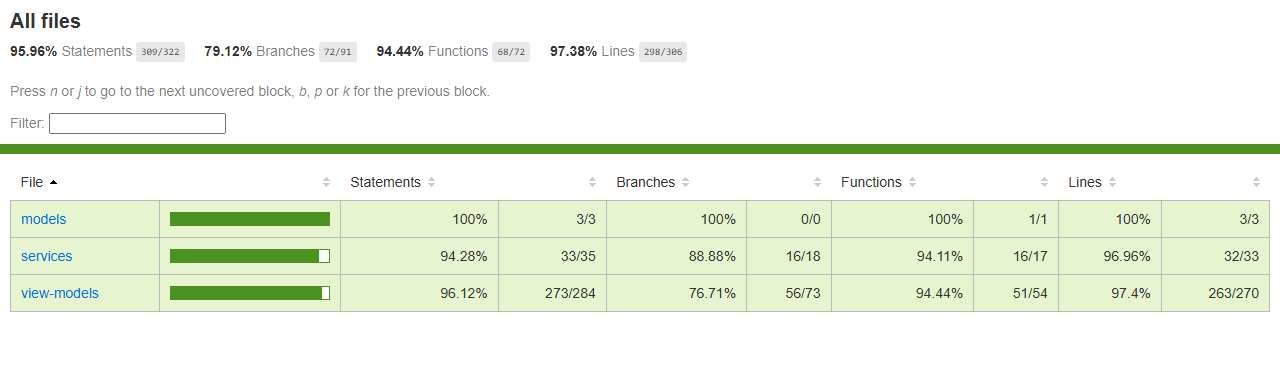
\includegraphics[width=\textwidth]{imagens/coverage-frontend.png}
\par\vspace{0.5em}
\parbox{\textwidth}{\raggedright\small\textit{Fonte: Elaborado pelo Autor (2026).}}
\end{figure}

Conforme ilustrado, o frontend atingiu 82,6\% de cobertura de comandos (\textit{Statements}), 65,38\% de ramos (\textit{Branches}), 83,33\% de funções (\textit{Functions}) e 83,66\% de linhas (\textit{Lines}). O \texttt{useEditCertificateViewModel.ts} passou de 0\% para 95,55\% em comandos e 100\% em funções após a inclusão de testes. O \texttt{schemas.test.ts} recebeu 9 novos testes para o \texttt{updateCertificateSchema}, abrangendo validação de CPF e campos obrigatórios. Os únicos ramos não cobertos (65,38\%) são os guards \texttt{if (!active)} no \texttt{useEffect} --- um aborto que só ocorre se o componente desmontar antes do \textit{fetch}, caso raro e aceitável.

\subsubsection{Backend (CertifyHub Server)}

O backend contém 19 suítes de testes com 168 testes unitários, cobrindo casos de uso (emissão e reemissão \ref{rf:gerar-pdf}--\ref{rf:download-individual}, validação \ref{rf:portal-validacao}--\ref{rf:exibir-validacao}, templates \ref{rf:upload-templates}--\ref{rf:duplicar-templates}), entidades de domínio (\texttt{Certificate}, \texttt{Template}, \texttt{VerificationCode}), repositórios (Supabase), serviços (PDFKit) e \textit{middleware} de autenticação e \textit{rate limiting} — principais camadas da arquitetura limpa adotada no MVP.

A Figura~\ref{fig:coverage-backend} apresenta o relatório de cobertura gerado pelo Jest para o backend.

\begin{figure}[H]
\centering
\caption{Relatório de cobertura dos testes — backend}
\label{fig:coverage-backend}
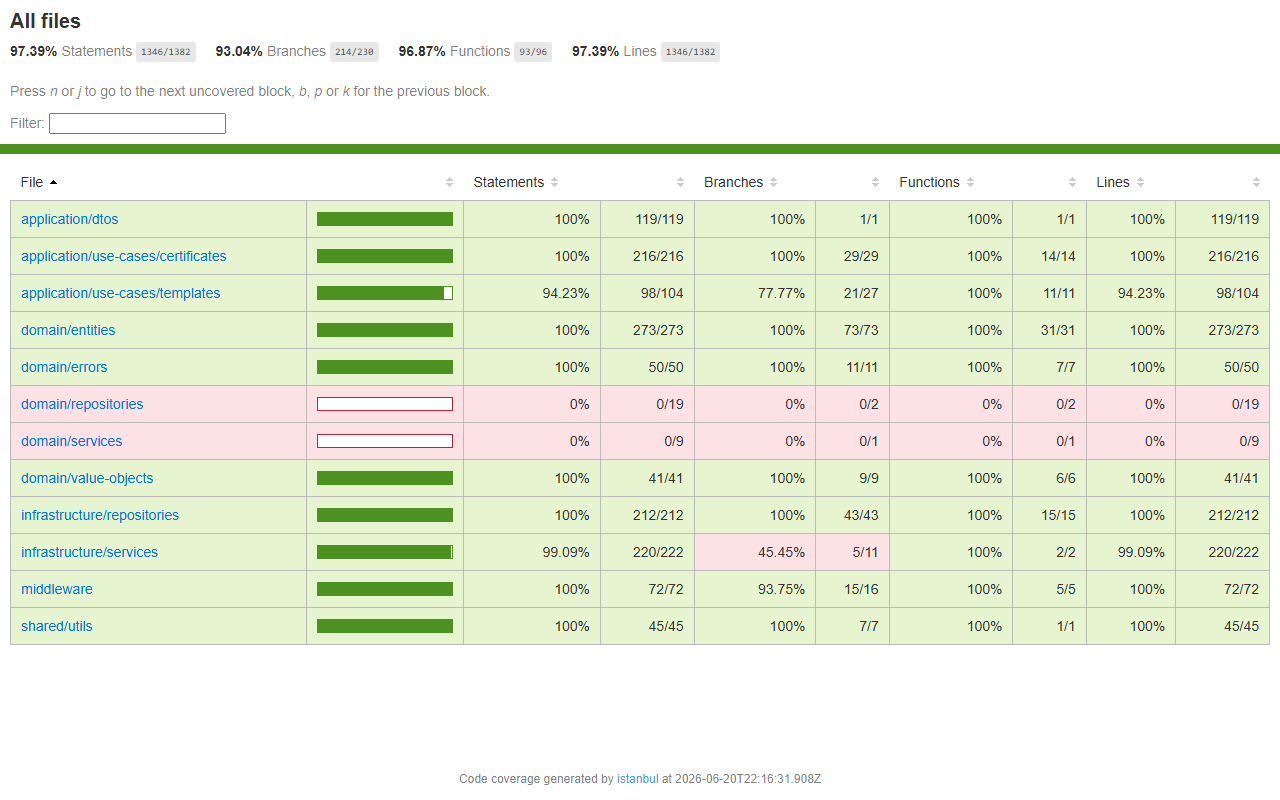
\includegraphics[width=\textwidth]{imagens/coverage-backend.png}
\par\vspace{0.5em}
\parbox{\textwidth}{\raggedright\small\textit{Fonte: Elaborado pelo Autor (2026).}}
\end{figure}

O backend atingiu 96,53\% de cobertura de comandos, 92,24\% de ramos, 95,87\% de funções e 96,53\% de linhas. As camadas de \textit{application/dtos}, \textit{domain/entities}, \textit{domain/errors}, \textit{domain/value-objects}, \textit{infrastructure/repositories}, \textit{middleware} e \textit{shared/utils} apresentaram cobertura integral (100\%), evidenciando que as regras de negócio e a lógica de persistência foram amplamente exercitadas pelos testes. A camada \textit{infrastructure/services} registrou 99,25\% em comandos e 41,66\% em ramos, diferença atribuída às condicionais de configuração do PDFKit que não foram totalmente cobertas. As interfaces \textit{domain/repositories} e \textit{domain/services} aparecem com 0\% por se tratarem de contratos abstratos (interfaces) sem implementação concreta a ser testada diretamente.

\subsubsection{Testes End-to-End}
\label{subsubsec:e2e}

Para validar a integração entre frontend e backend em cenário realista, foi implementado um teste \textit{end-to-end} com Playwright que percorre o fluxo completo: criar um template, emitir um certificado, verificar a autenticidade pela página pública e, ao final, excluir o certificado — contemplando também o fluxo de remoção com confirmação via \texttt{confirm()}. O teste é executado contra o servidor de desenvolvimento local (Vite na porta 5173) e depende do backend rodando simultaneamente (Next.js na porta 3000). Todo o processo é orquestrado automaticamente pelo Playwright, que inicia o frontend via \texttt{npm run dev} antes da execução. A suíte inclui também um \textit{script} auxiliar de população de dados (\texttt{popular.spec.ts}), utilizado apenas para preparar o ambiente de demonstração, totalizando 2 arquivos de especificação na Figura~\ref{fig:e2e-report}. O tempo total de execução, conforme o relatório gerado pelo Playwright, foi de 8,43\,s — incluindo ambos os \textit{scripts} executados em paralelo com 2 \textit{workers}.

O teste demonstra que o sistema suporta o fluxo crítico de ponta a ponta sem intervenção manual. Durante o desenvolvimento, foi identificado e corrigido um erro de configuração de CORS no backend (\texttt{next.config.ts}), que impedia a comunicação entre os serviços em \texttt{localhost}. A Figura~\ref{fig:e2e-report} apresenta o relatório gerado pelo Playwright, que exibe o passo a passo da execução, incluindo as capturas de tela de cada etapa e o resultado final (aprovado). O \textbf{CT057} (validação via \textit{QR Code}) permanece como \textbf{Planejado} -- embora a geração do \textit{QR Code} no PDF já esteja implementada no backend (\texttt{PDFKitService.ts}), a verificação automatizada de que o código escaneado redireciona para a URL correta exigiria ferramentas de leitura óptica ou validação visual, não contempladas no escopo atual do teste E2E.

\begin{figure}[H]
\centering
\caption{Relatório do teste \textit{end-to-end} gerado pelo Playwright}
\label{fig:e2e-report}
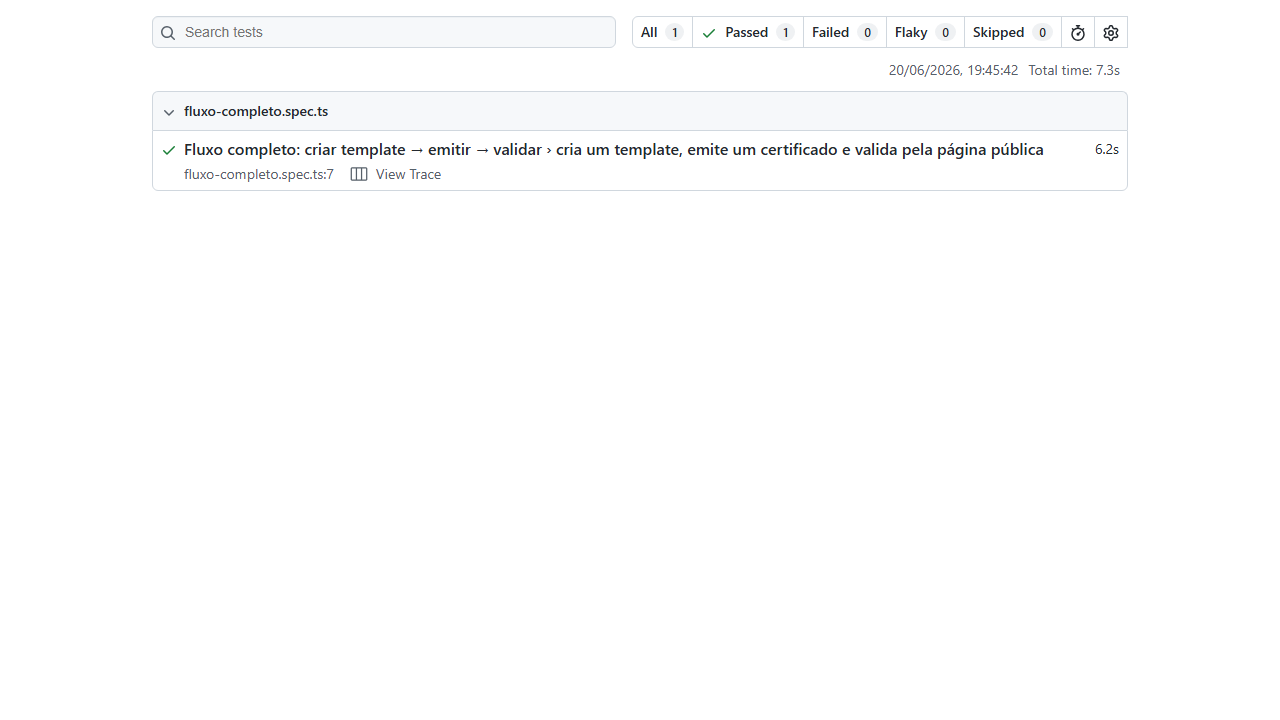
\includegraphics[width=\textwidth]{imagens/e2e-report.png}
\par\vspace{0.5em}
\parbox{\textwidth}{\raggedright\small\textit{Fonte: Elaborado pelo Autor (2026).}}
\end{figure}

\subsubsection{Limitações}

Embora a cobertura geral tenha atingido percentuais elevados, algumas limitações devem ser registradas. Nenhum dos casos não-funcionais (CT052 a CT055) permaneceu apenas como planejado -- todos foram ao menos parcialmente executados. O \textbf{CT052} (carga -- geração simultânea de PDFs) foi executado com 10 chamadas concorrentes, porém sem variação de carga ou teste de estresse. O \textbf{CT053} (segurança -- acesso não autenticado) e o \textbf{CT054} (segurança -- força bruta) foram integralmente executados com testes automatizados no \textit{middleware} de autenticação e \textit{rate limiting}. O \textbf{CT055} (acessibilidade -- navegação por teclado) foi executado de forma limitada, restrito à navegação Tab entre dois campos do formulário de edição de validade; não há auditoria automatizada com ferramentas como \texttt{axe-core}. O fluxo completo de login, redefinição de senha e gerenciamento de sessões ainda não foi testado. Testes de integração com o banco de dados Supabase não foram realizados -- os repositórios foram testados com o cliente Supabase \textit{mockado}. O teste E2E atualmente cobre apenas o fluxo principal (\textit{happy path}); cenários de erro, como template ausente ou CPF inválido, não são abordados. O \textbf{CT057} (validação via \textit{QR Code}) não foi implementado como teste automatizado -- a funcionalidade de geração do \textit{QR Code} no PDF está implementada, porém a verificação de que o código escaneado redireciona para a URL de validação correta exigiria leitura óptica automatizada ou validação visual, sendo postergado para versões futuras. Cenários de carga e desempenho foram testados apenas para geração de PDF, não para os demais \textit{endpoints}. Essas lacunas representam oportunidades de melhoria para versões futuras do sistema.

\subsubsection{Resumo Geral}

A Tabela~\ref{tab:testes-resumo} consolida os resultados dos testes em ambos os módulos, incluindo as métricas de cobertura. Ambos os módulos superam o limiar mínimo de 75\% de cobertura definido na configuração do Jest e validado no pipeline de CI.

\begin{table}[H]
\centering
\caption{Resumo geral dos testes}
\label{tab:testes-resumo}
\begin{tabularx}{\textwidth}{Xcccc}
\toprule
\textbf{Módulo} & \textbf{Suítes} & \textbf{Testes} & \textbf{Cobertura} & \textbf{Tempo} \\
\midrule
Frontend (CertifyHub) & 13 & 121 & 82,6\% & 38,57\,s \\
Backend (CertifyHub Server) & 19 & 168 & 96,53\% & 14,86\,s \\
E2E (Playwright) & 1 & 1 & -- & 8,43\,s \\
\midrule
\textbf{Total} & \textbf{33} & \textbf{290} & \textbf{--} & \textbf{61,86\,s} \\
\bottomrule
\end{tabularx}
\par\vspace{6pt}
\mbox{}\vspace{6pt}\par
\footnotesize\noindent\textbf{Nota:} Os 290 testes automatizados (121 + 168 + 1 E2E) referem-se exclusivamente aos testes unitários, de integração e \textit{end-to-end}. Desses, 4 são casos de teste não-funcionais (CT052 a CT055): CT052 (carga) possui teste automatizado no backend com 10 chamadas concorrentes em \textless 5s; CT053 (autenticação) e CT054 (\textit{rate limiting}) foram integralmente automatizados no \textit{middleware}; CT055 (acessibilidade) possui teste automatizado de navegação Tab no frontend, porém sem auditoria com ferramentas como \texttt{axe-core}.
\par\vspace{4pt}
\end{table}
\noindent\raggedright\small\textit{Fonte: Elaborado pelo Autor (2026).}


% CONSIDERAÇÕES FINAIS
\section{CONSIDERAÇÕES FINAIS}

Este capítulo apresenta as conclusões consolidadas ao longo do desenvolvimento do sistema, retomando os objetivos propostos na Seção~\ref{sec:objetivos} e avaliando em que medida foram alcançados. Além disso, destacam-se as principais contribuições técnicas do trabalho, as restrições identificadas no escopo atual e as perspectivas para evolução contínua da arquitetura.

O objetivo geral deste trabalho consistiu em projetar e implementar um sistema web automatizado para emissão, gestão e validação pública de certificados. O produto de software foi desenvolvido com êxito, resultando em um Produto Mínimo Viável (MVP) funcional, testado e alinhado aos requisitos de negócio. Através do acesso via navegador, a plataforma fornece funcionalidades robustas de emissão, gerenciamento de \textit{templates} visuais, \textit{dashboard} gerencial e um portal público de validação. O disparo automático de e-mails não foi implementado no escopo do MVP; a distribuição dos PDFs ocorre via canais institucionais convencionais (como e-mail manual ou compartilhamento de link), enquanto a geração dos certificados e o portal de validação já atendem ao fluxo principal do sistema. Sob a ótica da engenharia de software, conclui-se que o objetivo central foi plenamente atingido.

Em relação aos objetivos específicos propostos:

\begin{itemize}
    \item O módulo de \textbf{\textit{templates} configuráveis} foi concebido com um editor visual \textit{inline} e renderização em tempo real, permitindo personalização dinâmica de atributos visuais (\ref{rf:upload-templates}, \ref{rf:personalizacao-templates});
    \item O \textbf{mecanismo de autenticação pública}, ancorado em códigos únicos e \textit{QR Codes}, foi integrado ao portal de validação, mitigando riscos de fraudes e falsificações (\ref{rf:portal-validacao}, \ref{rf:validar-certificado});
    \item O \textbf{\textit{dashboard} com indicadores gerenciais} foi implantado, fornecendo telemetria sobre estatísticas de emissão, certificados ativos e uso de \textit{templates} (\ref{rf:estatisticas-emissao});
    \item A \textbf{qualidade do software} foi assegurada através de uma suíte abrangente de \textbf{testes automatizados}, englobando testes unitários (atingindo cobertura de 82,6\% no \textit{frontend} e 96,53\% no \textit{backend}) e \textit{end-to-end}, devidamente integrados ao \textit{pipeline} de integração contínua (Seção~4.3);
    \item O \textbf{ambiente de implantação} foi orquestrado em infraestrutura em nuvem (Render), adotando \textit{pipelines} de Integração e Entrega Contínuas (CI/CD) nativos a partir do GitHub, garantindo \textit{deploys} contínuos e resilientes (Seção~4.1).
\end{itemize}

Devido à adoção da abordagem iterativa e às restrições inerentes ao escopo de um MVP, alguns objetivos específicos foram estrategicamente postergados para iterações futuras. O suporte a importação de dados em lote via arquivos (CSV e Excel) e o serviço de mensageria para envio automático de e-mails não foram incorporados ao \textit{backend} nesta versão. Adicionalmente, os mecanismos rígidos de conformidade com a LGPD e a implementação integral da arquitetura \textit{multi-tenant} requerem validações jurídicas e de infraestrutura, sendo mapeados como evoluções necessárias para o \textit{roadmap} futuro.

\subsection{PRINCIPAIS CONTRIBUIÇÕES}

O sistema desenvolvido oferece uma solução tecnológica moderna e eficiente para o problema identificado, cujas principais contribuições são:

\begin{itemize}
    \item \textbf{Digitalização do fluxo de emissão:} a transição de ferramentas de escritório genéricas para um fluxo automatizado e dedicado reduz a fricção operacional, mitigando falhas humanas e retrabalho;
    \item \textbf{Verificabilidade e Transparência:} a introdução de um portal público, acessível via \textit{QR Code}, descentraliza o processo de auditoria de certificados, provendo verificação em tempo real sem ônus operacional para a instituição emissora;
    \item \textbf{Governança de Dados:} a persistência de registros de emissão em banco de dados relacional com carimbo de tempo e autoria garante rastreabilidade total do ciclo de vida dos certificados;
    \item \textbf{Arquitetura Desacoplada e Escalável:} a segregação entre \textit{frontend} (Vite/React) e \textit{backend} (Next.js), orientada a princípios de arquitetura limpa, promove alta coesão, testabilidade e facilita a evolução independente dos microsserviços;
    \item \textbf{Esteira de CI/CD Automatizada:} a implementação de fluxos de CI/CD garante que todo incremento de código seja automaticamente testado (lint, tipo, unitário, integração e E2E) antes de atingir o ambiente de produção.
\end{itemize}

\subsection{LIMITAÇÕES}

Do ponto de vista arquitetural e funcional, o produto atual apresenta as seguintes limitações, oriundas de \textit{trade-offs} assumidos no escopo do MVP:

\begin{itemize}
    \item O fluxo de \textbf{emissão em lote} é atualmente sequencial e manual na interface; a ausência de um \textit{message broker} (processamento em fila) e de suporte à importação de arquivos (CSV/Excel) limita o rendimento para volumes massivos de dados;
    \item A \textbf{notificação ativa (E-mail)} não foi implementada no lado do servidor (sem integração com provedores SMTP). O artefato atual no \textit{frontend} (\code{envios.ts}) apenas estrutura o agendamento em armazenamento local (\code{localStorage}) de forma simulada;
    \item A \textbf{arquitetura \textit{multi-tenant}} não foi finalizada -- o banco de dados opera sob o paradigma de \textit{tenant} único, sem o particionamento lógico de dados essencial para um modelo SaaS em larga escala;
    \item A \textbf{adequação à LGPD} carece de refinamento -- mecanismos como ofuscação/anonimização de dados pessoais e gestão granular de consentimento ainda não estão materializados no código;
    \item A \textbf{reemissão com manutenção de histórico} (\ref{rf:reemissao-historico}) não foi implementada -- a edição de certificados sobrescreve os dados in-place, sem gerar novo código de verificação ou preservar a versão anterior;
    \item A \textbf{autenticação via JWT com Supabase Auth} não foi integralmente implementada -- o middleware de autenticação existe no backend e foi validado em testes unitários, mas o fluxo completo de login, gerenciamento de sessão e renovação de tokens está previsto para versões futuras;
    \item A suíte de testes carece de \textbf{testes de carga e estresse}, os quais são fundamentais para atestar o comportamento e as garantias do serviço de geração de PDFs sob alta concorrência.
\end{itemize}

\subsection{TRABALHOS FUTUROS}

Vislumbrando a evolução contínua da plataforma, recomenda-se a exploração dos seguintes aprimoramentos técnicos e funcionais:

\begin{itemize}
    \item Materialização das entidades \textbf{PARTICIPANTES} e \textbf{CURSOS} no banco de dados, substituindo a abordagem denormalizada atual (campos \code{recipientName}, \code{recipientCPF}, \code{courseName} e \code{courseHours} diretamente na tabela \code{CERTIFICADOS}) por um modelo relacional normalizado com chaves estrangeiras (\code{participantId} e \code{courseId}), habilitando histórico de certificados por participante, listagem por curso e relatórios gerenciais por unidade de treinamento;
    \item Adoção de um \textbf{serviço de mensageria / fila} (como Redis/BullMQ ou RabbitMQ) para orquestrar o processamento assíncrono de emissões em lote e processamento de arquivos CSV/Excel;
    \item Integração com provedores de nuvem para \textbf{envio transacional de e-mails}, implementando retentativas exponenciais (\textit{exponential backoff}) e \textit{templates} ricos;
    \item Refatoração do modelo de dados para suportar plenamente o \textbf{isolamento \textit{multi-tenant}}, com políticas de segurança de linha (\textit{Row Level Security} - RLS) via Supabase;
    \item Implementação nativa de um módulo de \textbf{auditoria e conformidade com a LGPD}, incorporando \textit{logs} imutáveis e fluxos automatizados para a exclusão de dados pessoais;
    \item Execução de campanhas de \textbf{testes não-funcionais} (carga/desempenho) e \textbf{análise automatizada de vulnerabilidades} na esteira de CI/CD, com ênfase em patamares de concorrência superiores (50, 100 e 500 requisições simultâneas) para o serviço de geração de PDF, validando o comportamento do sistema sob carga real de produção;
    \item Investigação sobre a viabilidade de ancoragem criptográfica dos certificados através de \textbf{Assinatura Digital (ICP-Brasil)} ou redes \textbf{Blockchain}, visando segurança e imutabilidade incontestáveis;
    \item Implementação de \textbf{versionamento da API} (ex.: \texttt{/api/v1/}, \texttt{/api/v2/}), permitindo evolução sem quebrar contratos com clientes existentes e habilitando migração gradual entre versões.
\end{itemize}

% ================= REFERÊNCIAS =====================
\newpage
\bibliographystyle{abntex2-num-sentcase}
\bibliography{referencias}
\addcontentsline{toc}{section}{REFERÊNCIAS}

% ================= ANEXOS =================
\newpage

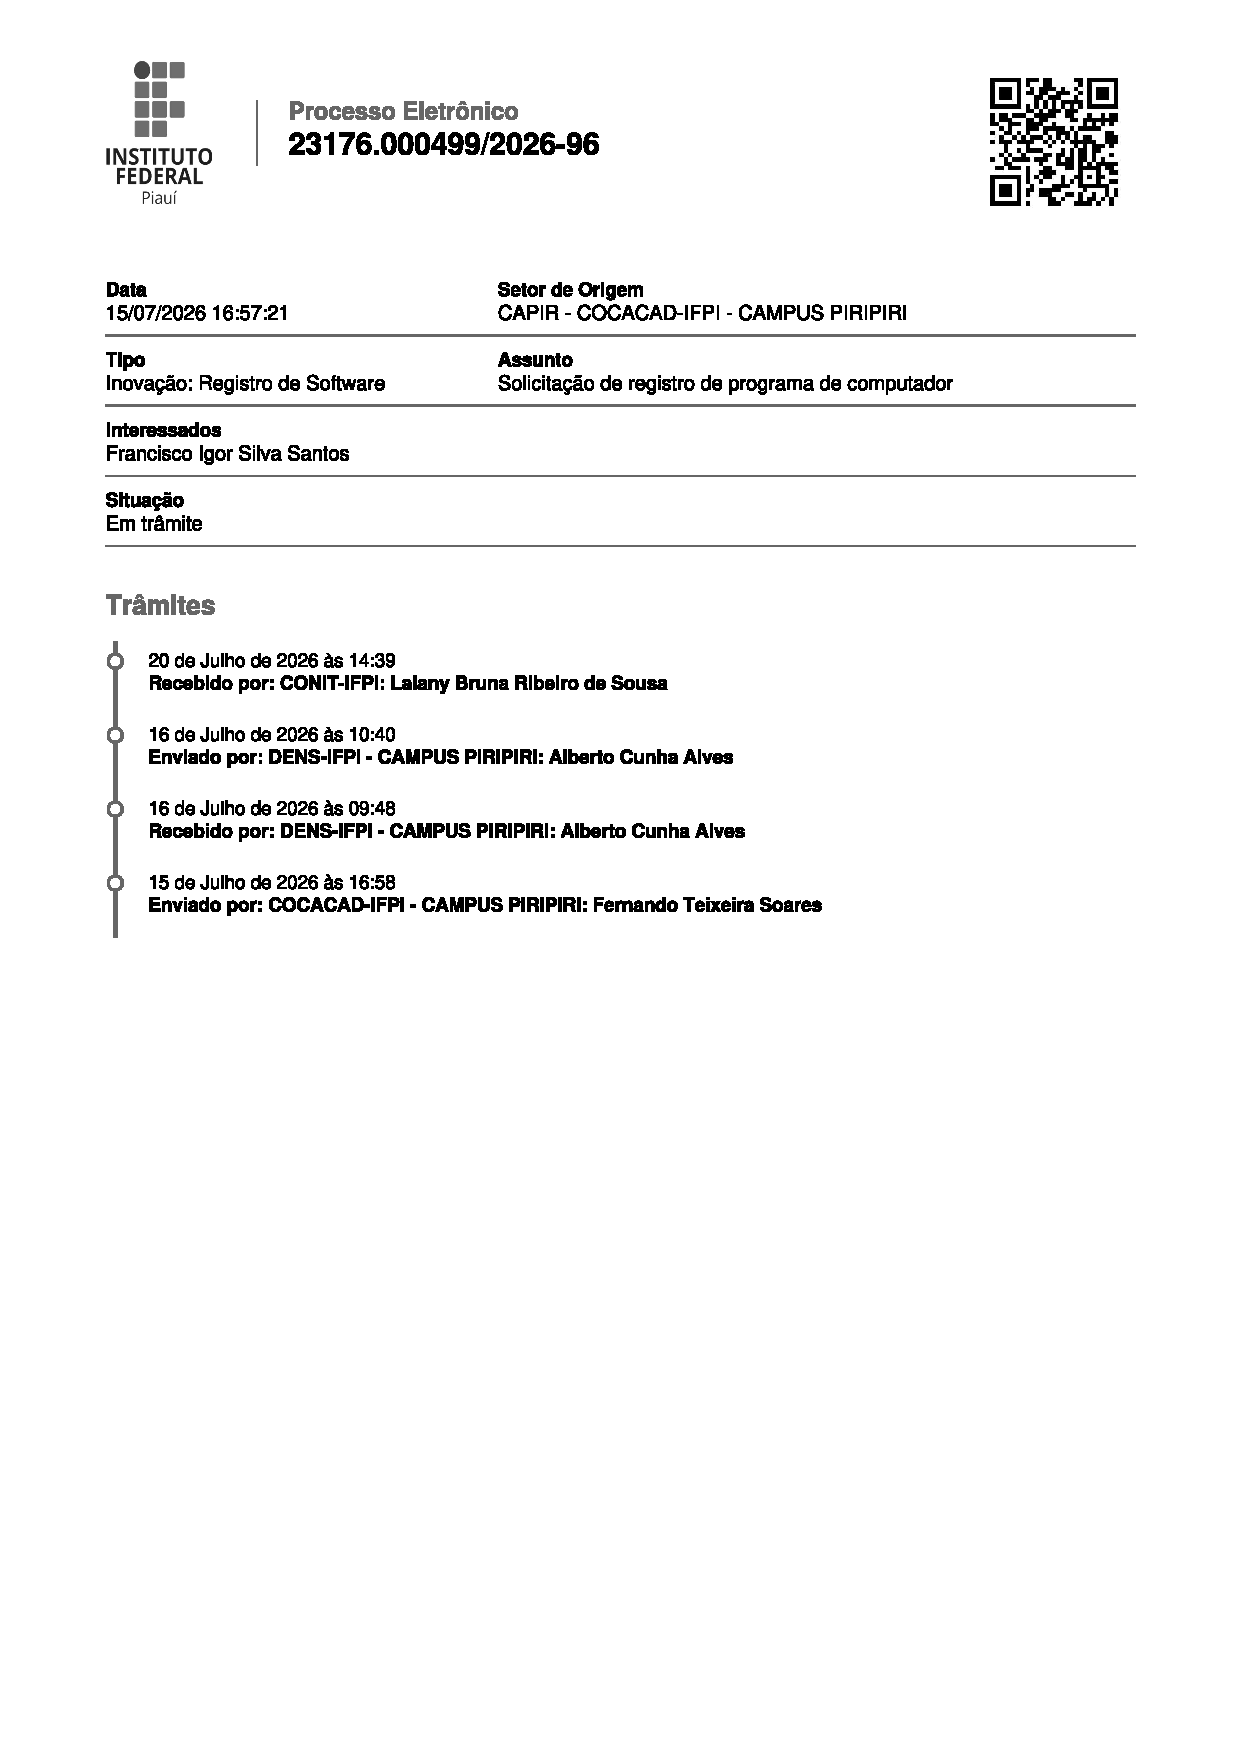
\includepdf[pages=-,width=\textwidth,trim=0 3cm 0 0,clip,pagecommand={\thispagestyle{fancy}\section{ANEXOS}\begin{center}\large\textbf{ANEXO A --- Declaração de Entrega do Código-Fonte}\end{center}\vspace{0.5cm}}]{anexos/Processo-requerimento.pdf}

\clearpage

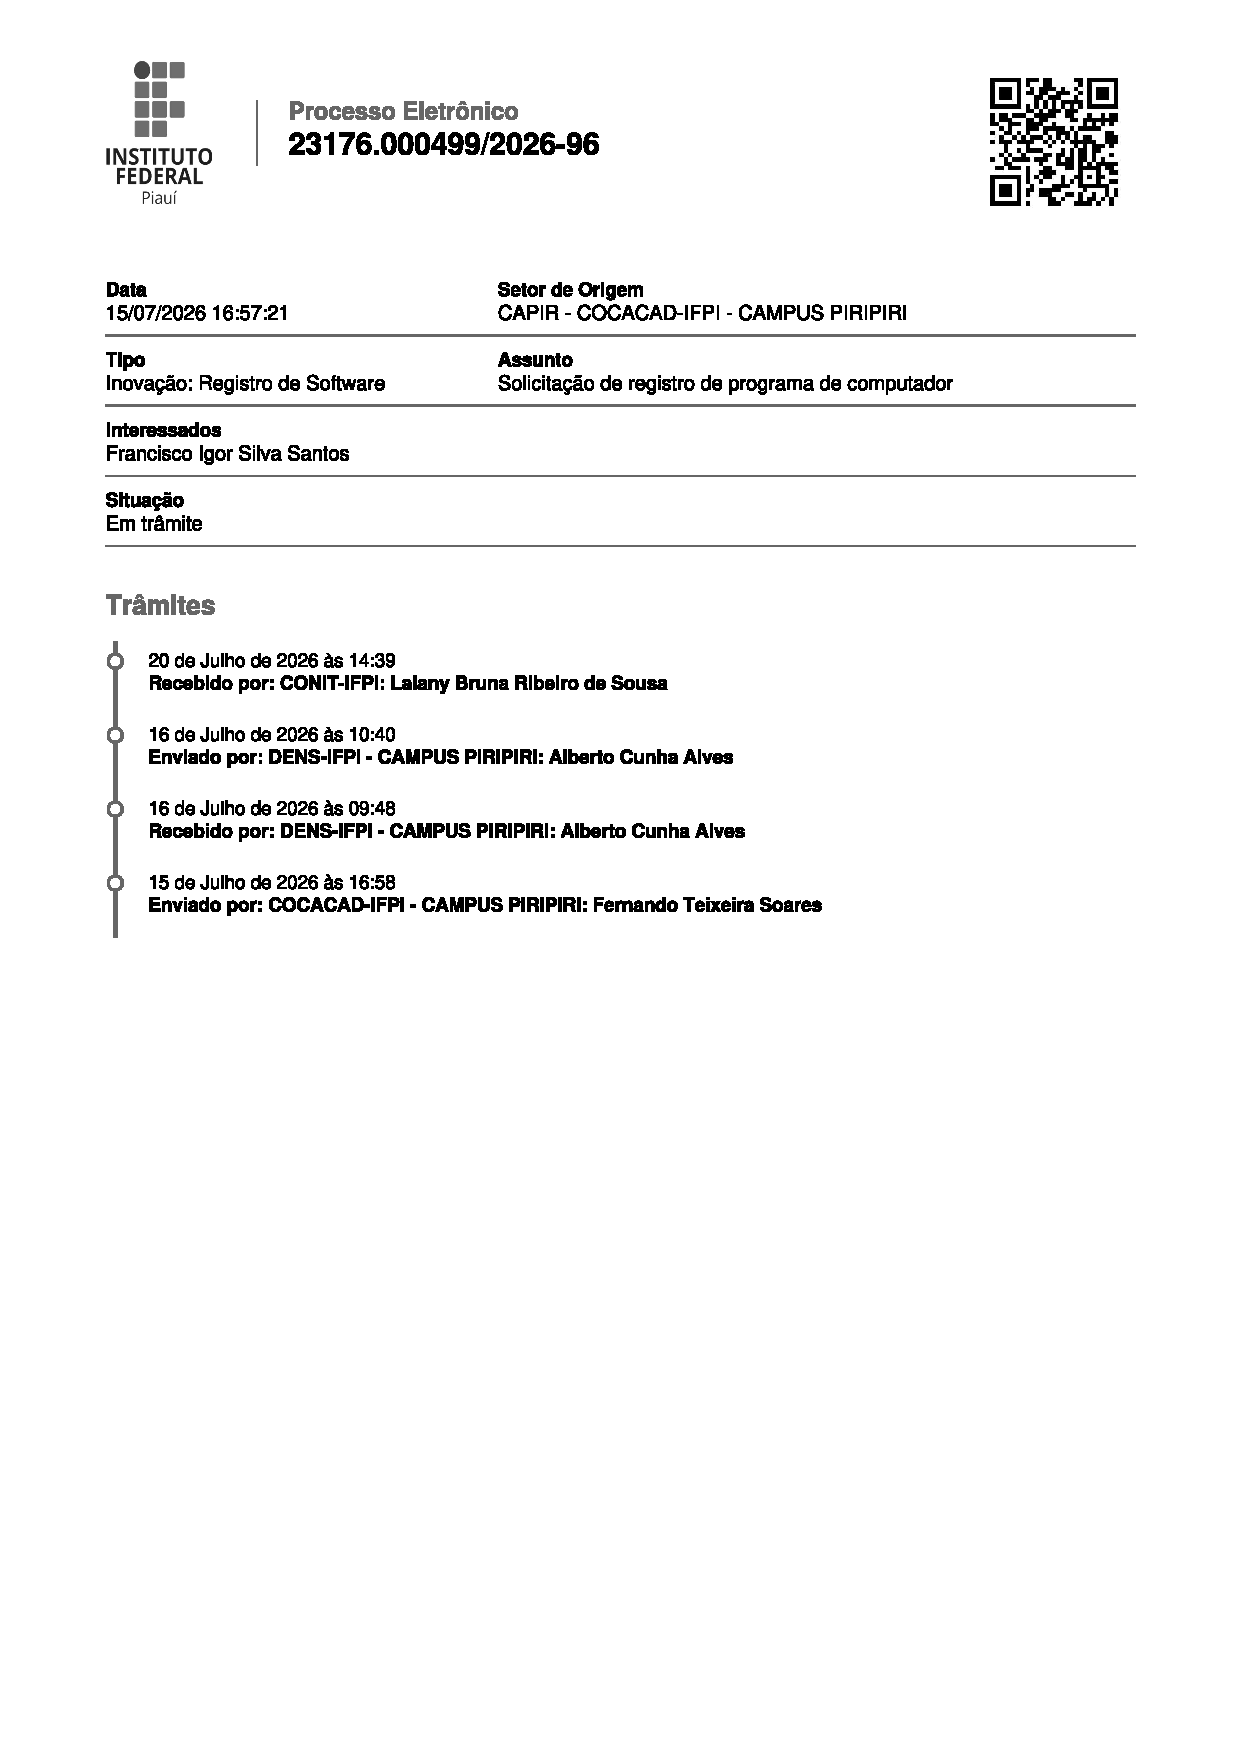
\includepdf[pages=-,width=\textwidth,trim=0 3cm 0 0,clip,pagecommand={\thispagestyle{fancy}\begin{center}\large\textbf{ANEXO B --- Declaração de Submissão ao NIT}\end{center}\vspace{0.5cm}}]{anexos/Processo-requerimento.pdf}

\end{document}
